\documentclass[beamer=true]{standalone}
\usepackage{../../preamblesnotes}

\begin{document}
\settitle{波動}{波動學第一課}{周末班}

\section{oscillation}
\begin{frame}{振動}
    % \par{\par\centering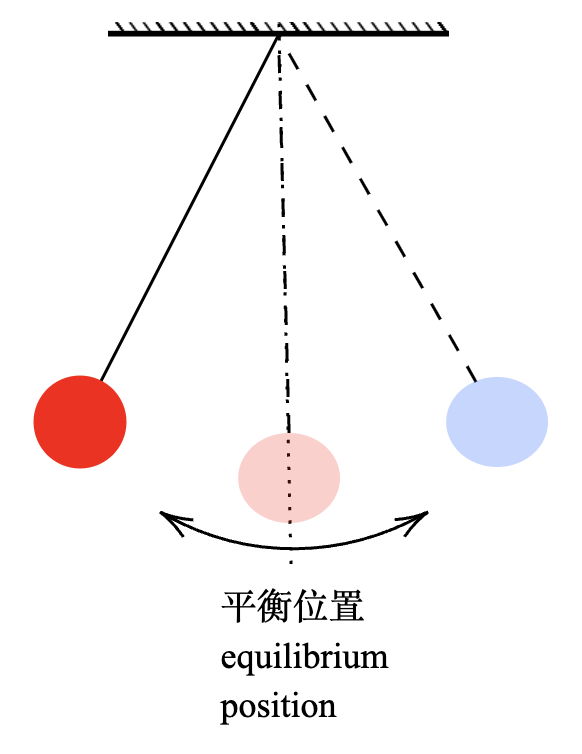
\includegraphics[width=.5\textwidth]{./img/ch1_2024-05-03-16-47-21.png}\par}
    \par{\par\centering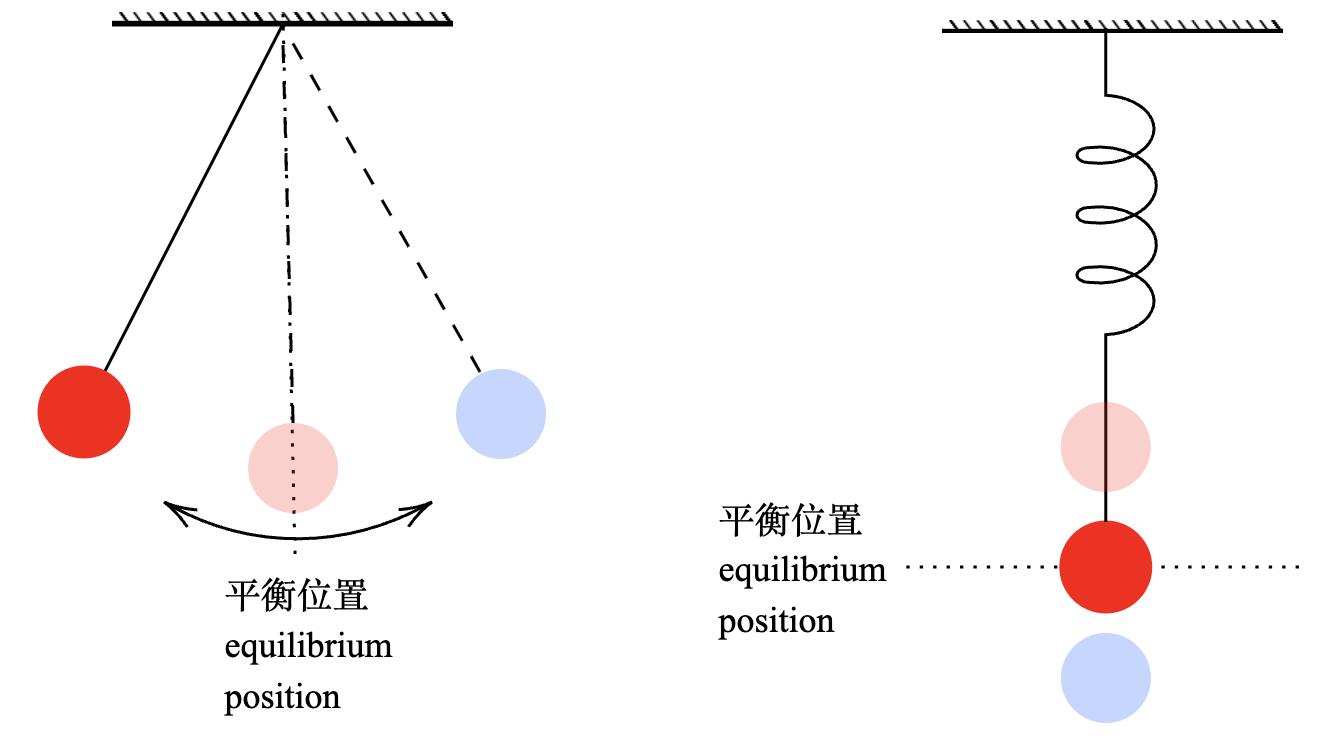
\includegraphics[width=\textwidth]{./img/ch1_2024-05-03-16-54-14.png}\par}
\end{frame}

\begin{frame}{振動}
    \begin{itemize}
        \item 振動過程是物件圍繞着一個\textbf{平衡位置}進行週期性運動。
        \item 在平衡位置中,物件的速率是最大值。
        \item 振動過程中也存在兩個極端位置,當中物件是\textbf{瞬時靜止}。
    \end{itemize}
\end{frame}

\begin{frame}{振動oscillation}
    % \par{\par\centering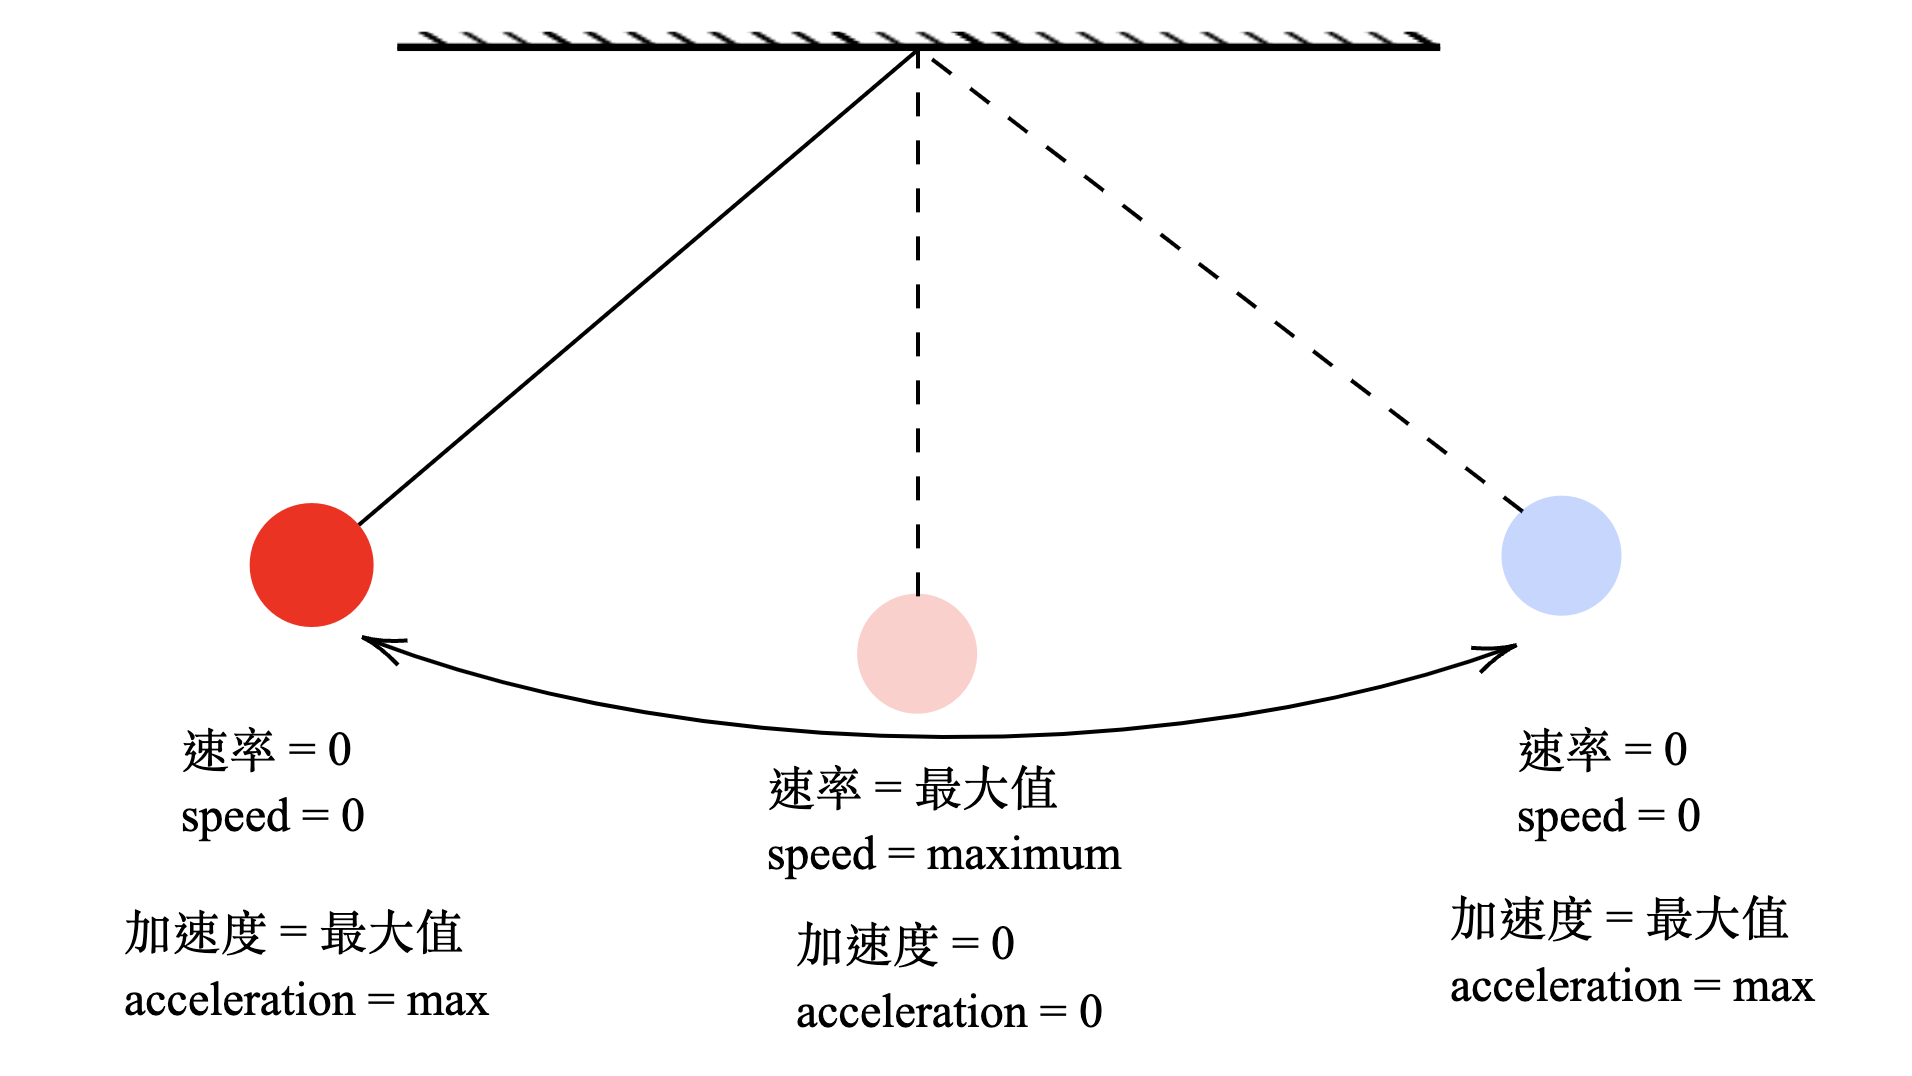
\includegraphics[width=\textwidth]{./img/ch1_2024-05-03-17-31-40.png}\par}
    % \par{\par\centering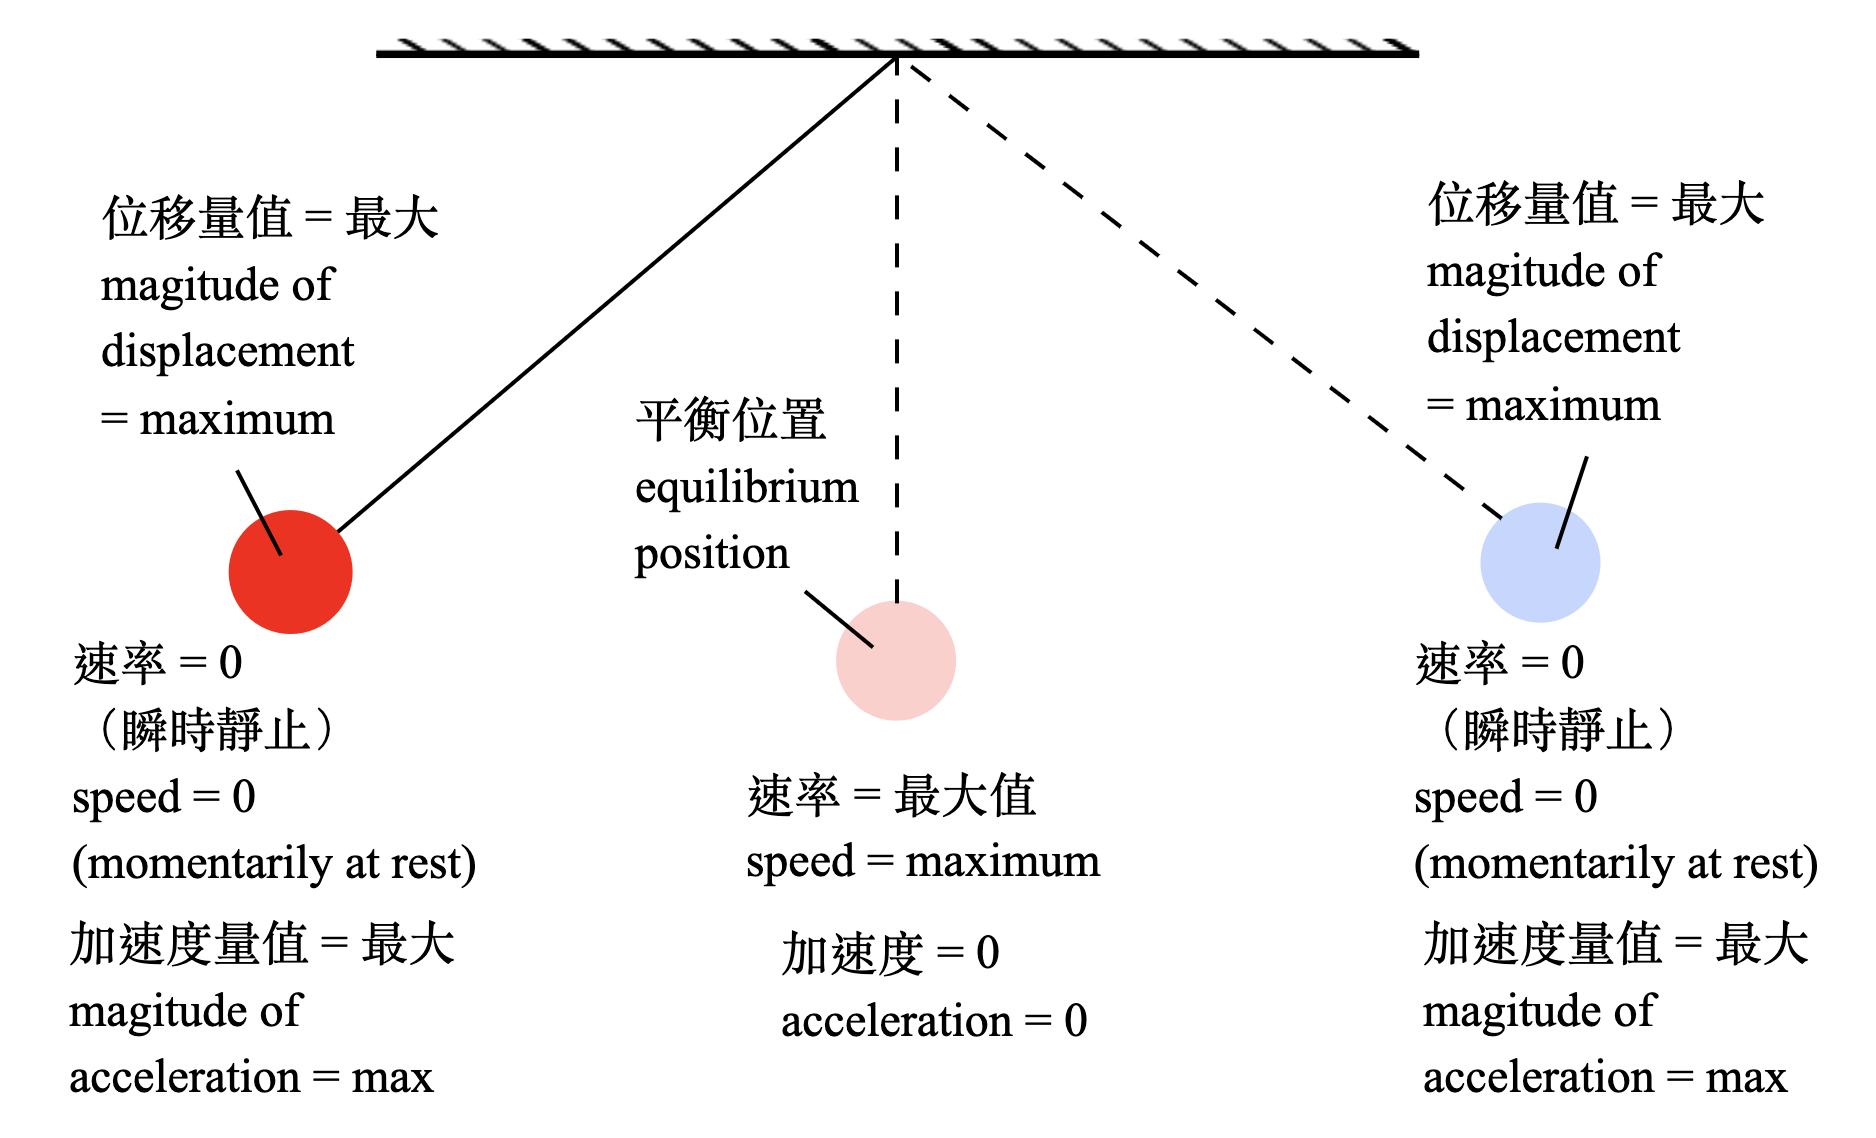
\includegraphics[width=\textwidth]{./img/ch1_2024-05-03-17-38-16.png}\par}
    \par{\par\centering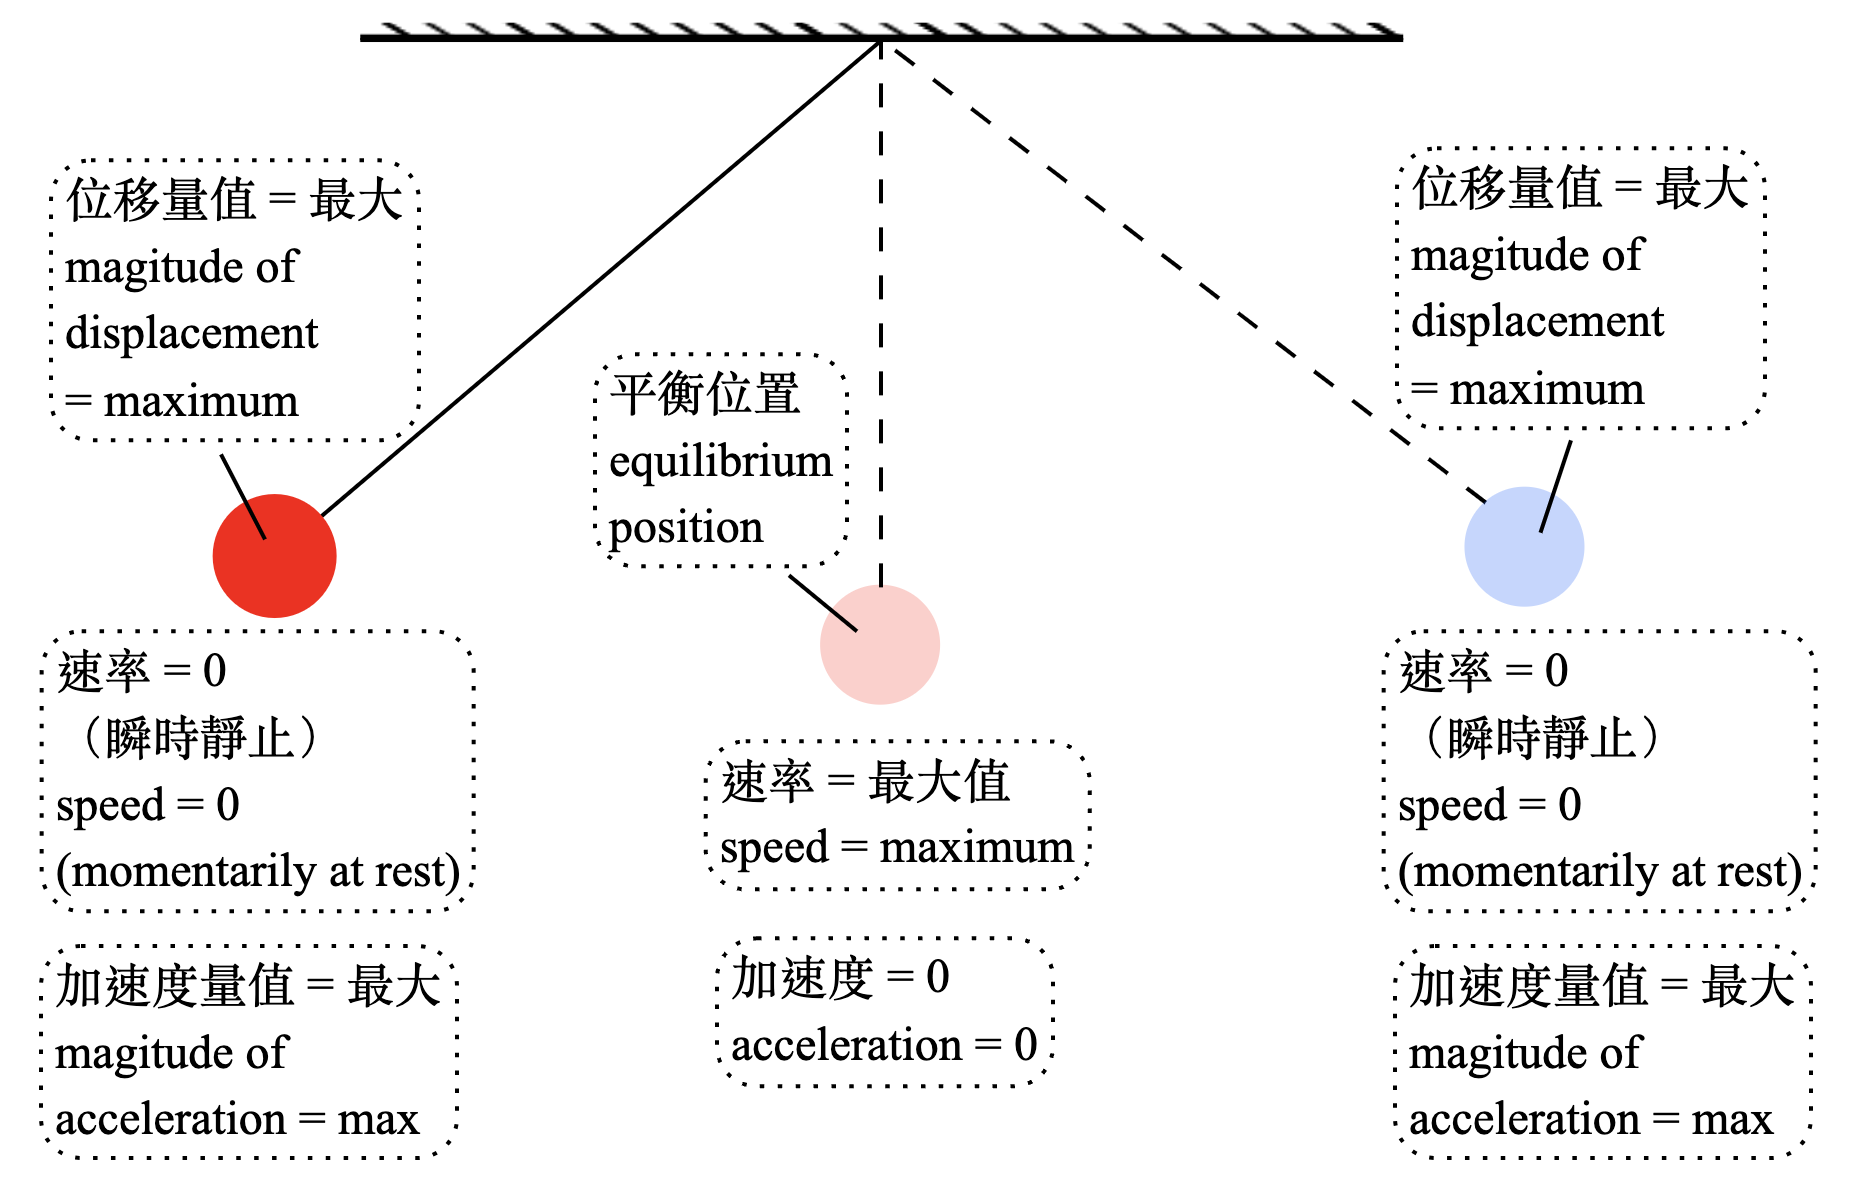
\includegraphics[width=\textwidth]{./img/ch1_2024-05-03-17-43-13.png}\par}
\end{frame}

\begin{frame}
    \frametitle{脈衝Pulse}
    \par{\par\centering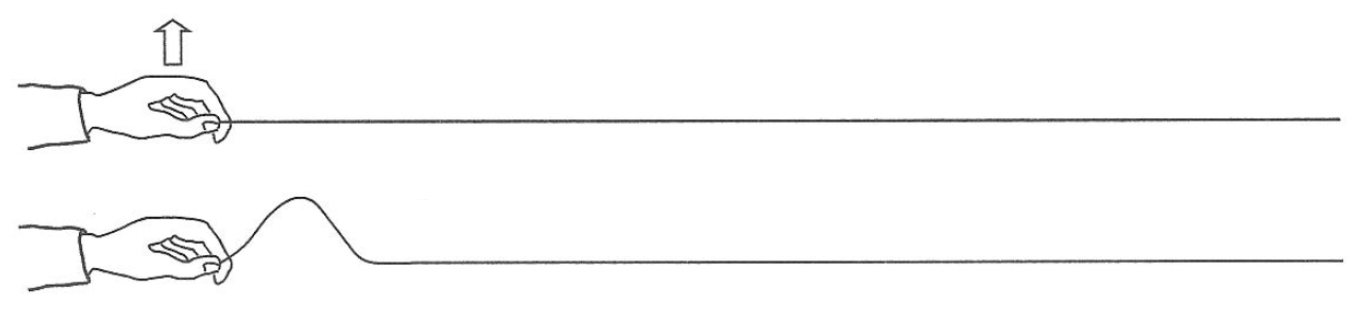
\includegraphics[width=.8\textwidth]{./img/ch1_2024-05-06-19-34-01.png}\par}
    \bigskip \bigskip
    \begin{itemize}
        \item 脈衝是一個持續短暫時間的波。\\A pulse of wave is a short duration of a wave.
        \item 如果給一條繩子一股脈衝,它會以固定的速率在繩子上移動。\\If a string is given a single disturbance, a pulse travels along the string with a steady speed.
    \end{itemize}
\end{frame}

\section{waves}
\begin{frame}{波動Wave}
    \begin{columns}
        \column{0.5\textwidth}
        \par{\par\centering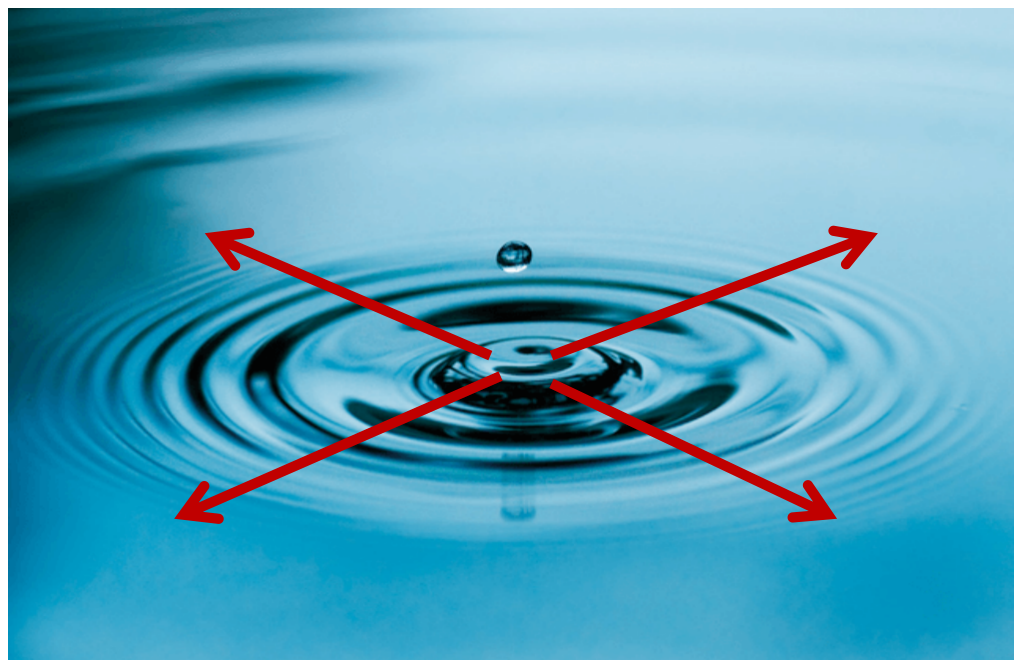
\includegraphics[width=.8\textwidth]{./img/ch1_2024-05-03-21-50-34.png}\par}\bigskip\bigskip
        \par{\par\centering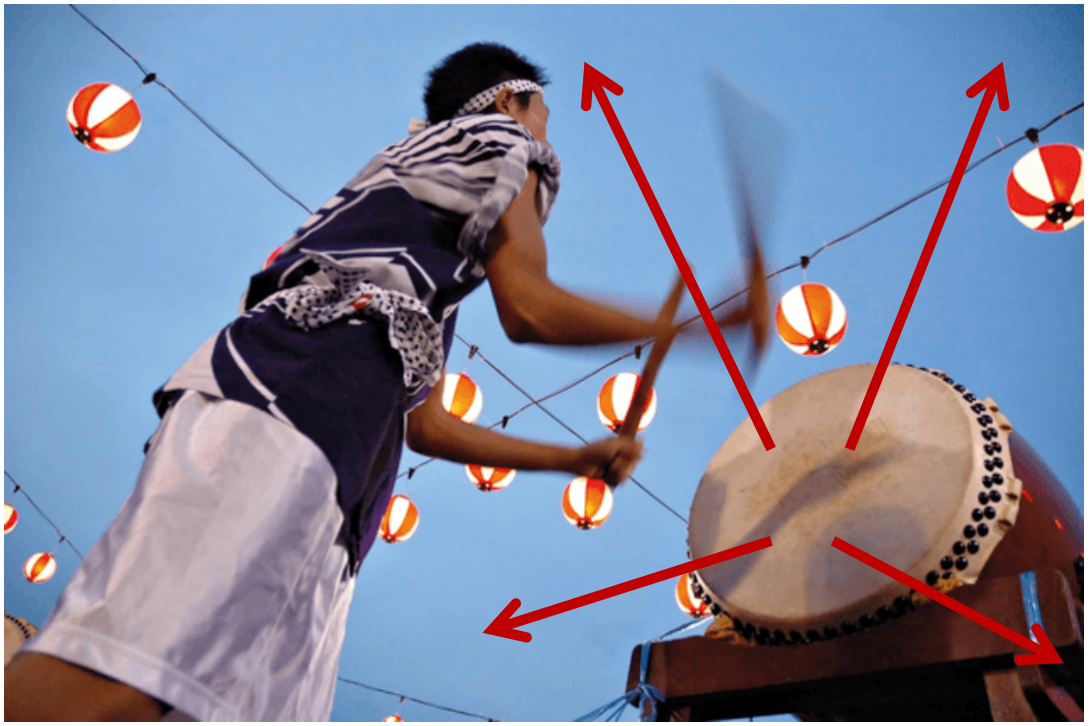
\includegraphics[width=.8\textwidth]{./img/ch1_2024-05-03-21-54-42.png}\par}
        \column{.5\textwidth}
        \par{\par\centering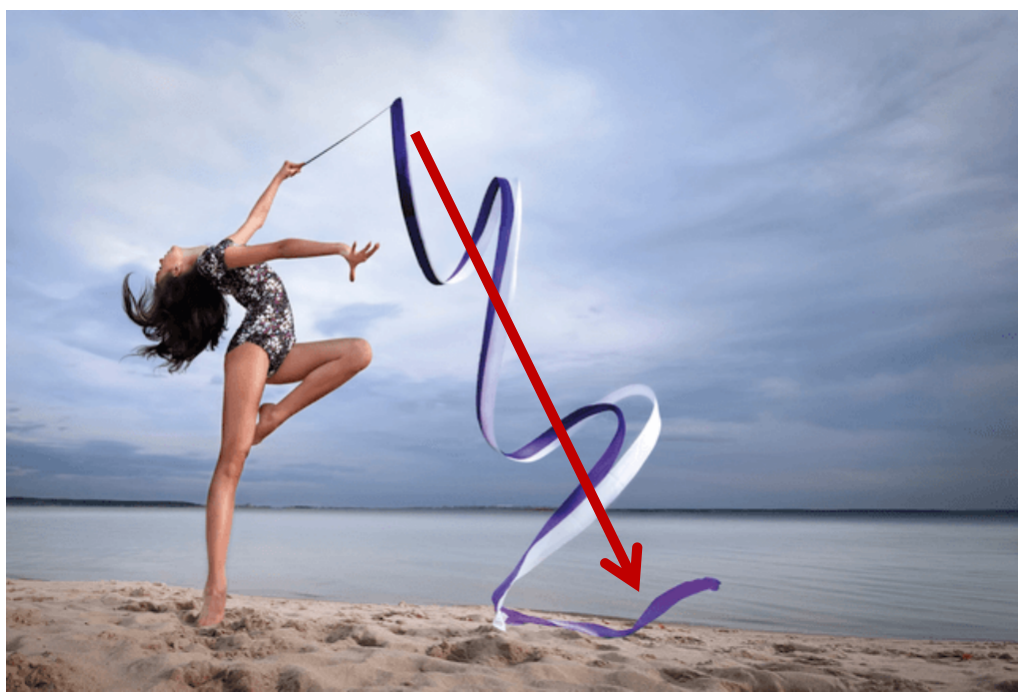
\includegraphics[width=.8\textwidth]{./img/ch1_2024-05-03-21-50-54.png}\par}\bigskip\bigskip
        \par{\par\centering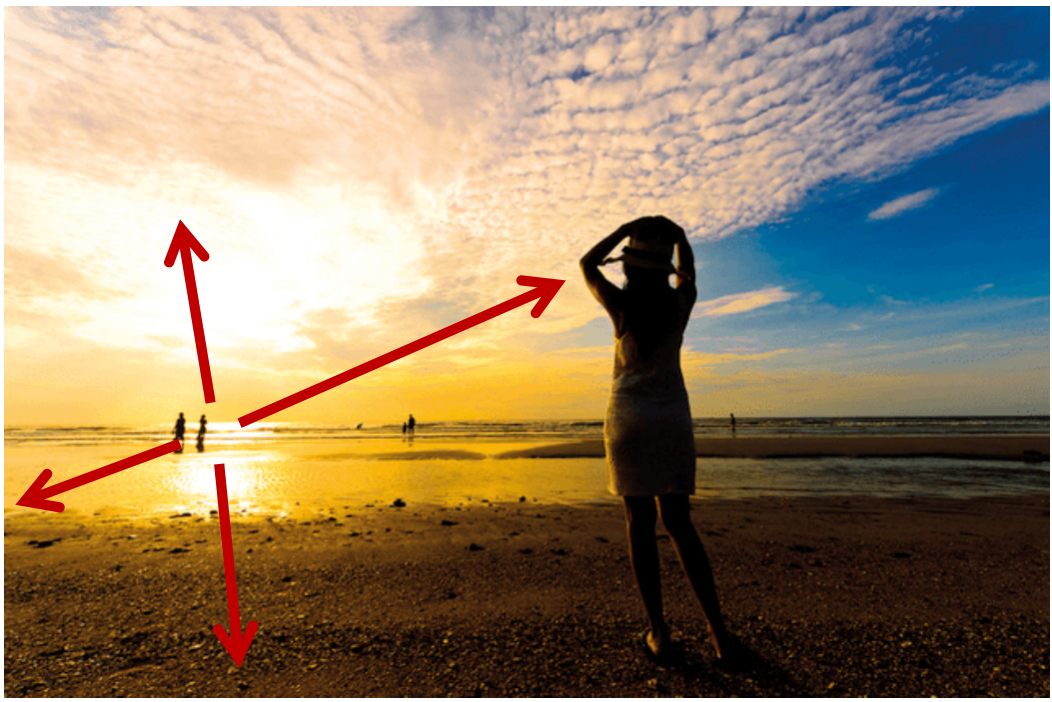
\includegraphics[width=.8\textwidth]{./img/ch1_2024-05-03-21-56-34.png}\par}
    \end{columns}
\end{frame}

\begin{frame}{波動的種類Types of waves}
    \begin{itemize}
        \item 波動是一種\textbf{能量的傳播}形式。\\Wave is a form of \textbf{propagation of energy.}
        \item 波動可分為\textbf{橫波}和\textbf{縱波}。\\Waves can be categorized into \textbf{transverse waves} and \textbf{longitudinal waves}.
        \item 橫波中,粒子的振動方向與波動的傳播方向互相\textbf{垂直}。\\In a transverse wave, the oscillation of the particles are \textbf{perpendicular} to the direction of propagation.
        \item 縱波中,粒子的振動方向與波動的傳播方向互相\textbf{平行}。\\In a longitudinal wave, the oscillation of the particles are \textbf{parallel} to the direction of propagation.
    \end{itemize}
\end{frame}

\begin{frame}{橫波和縱波Tranverse and longitudinal waves}
    \par{\par\centering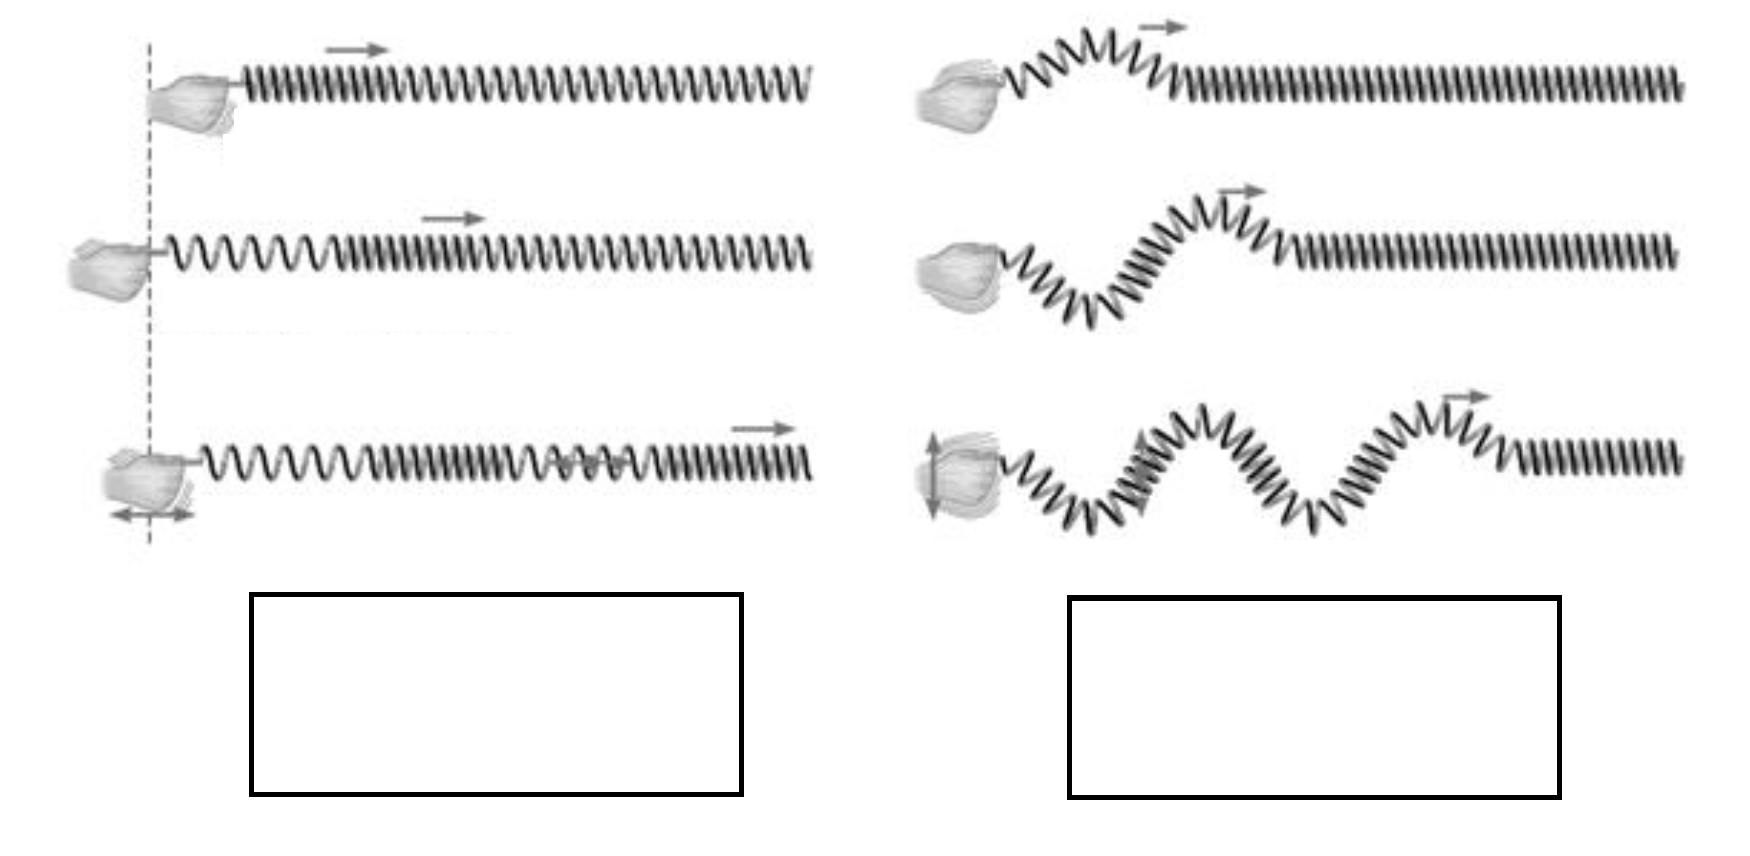
\includegraphics[width=\textwidth]{./img/ch1_2024-05-06-17-27-20.png}\par}
\end{frame}

\begin{frame}{機械波和電磁波 Mechanical and electromagnetic wave}
    \begin{columns}
        \column{.45\textwidth}
        \begin{exampleblock}
            {橫波的例子:\\Examples of transverse wave:}
            \begin{itemize}
                \item 水波 water wave
                \item 繩子上的波 \\wave on a string
                \item 地震波seismic wave
                \item 可見光 visible light
                \item 無線電波 radiowave
                \item 微波 microwave
                \item 紅外輻射 infrared radiation
                \item 紫外輻射 \\ultraviolet radiation
                \item X射線 X-ray
                \item 伽碼射線 $\gamma$ wave
            \end{itemize}
        \end{exampleblock}
        \column{.45\textwidth}
        \begin{exampleblock}
            {縱波的例子:\\Examples of longitudinal wave:}
            \begin{itemize}
                \item 彈簧上的波\\wave on a spring
                \item 聲波和超聲波\\sound wave
                \item 地震波seismic wave
            \end{itemize}
        \end{exampleblock}
    \end{columns}
\end{frame}

\begin{frame}{波動的種類Types of waves}
    \begin{itemize}
        \item 波動亦可分為機楲波和電磁波。\\On the other hand, waves can be categorized into mechanical waves and electromagnetic waves (EM waves).
        \item 對於\textbf{機械波}來說,波動的傳播需要\textbf{介質}。\\For a \textbf{mechanical wave}, it requires a \textbf{medium} to travel.
        \item 機械波的例子:\\Some examples of mechanical wave:
              \begin{itemize}
                  \item (橫波transverse wave)彈簧上的波  Wave on a spring
                  \item (橫波transverse wave)水波  Water wave
                  \item (縱波longitudinal wave)聲波 Sound wave
                  \item (橫+縱transverse + longitudinal)地震波 Seismic wave
              \end{itemize}
        \item 另一種波是\textbf{電磁波},不是機械波,它不需要介質來傳播。\\A non mechanical wave is called a \textbf{electromagnetic wave}, it does not require a medium to travel.
    \end{itemize}
\end{frame}

\begin{frame}{電磁波譜 Electromagetic spectrum}
    % \par{\par\centering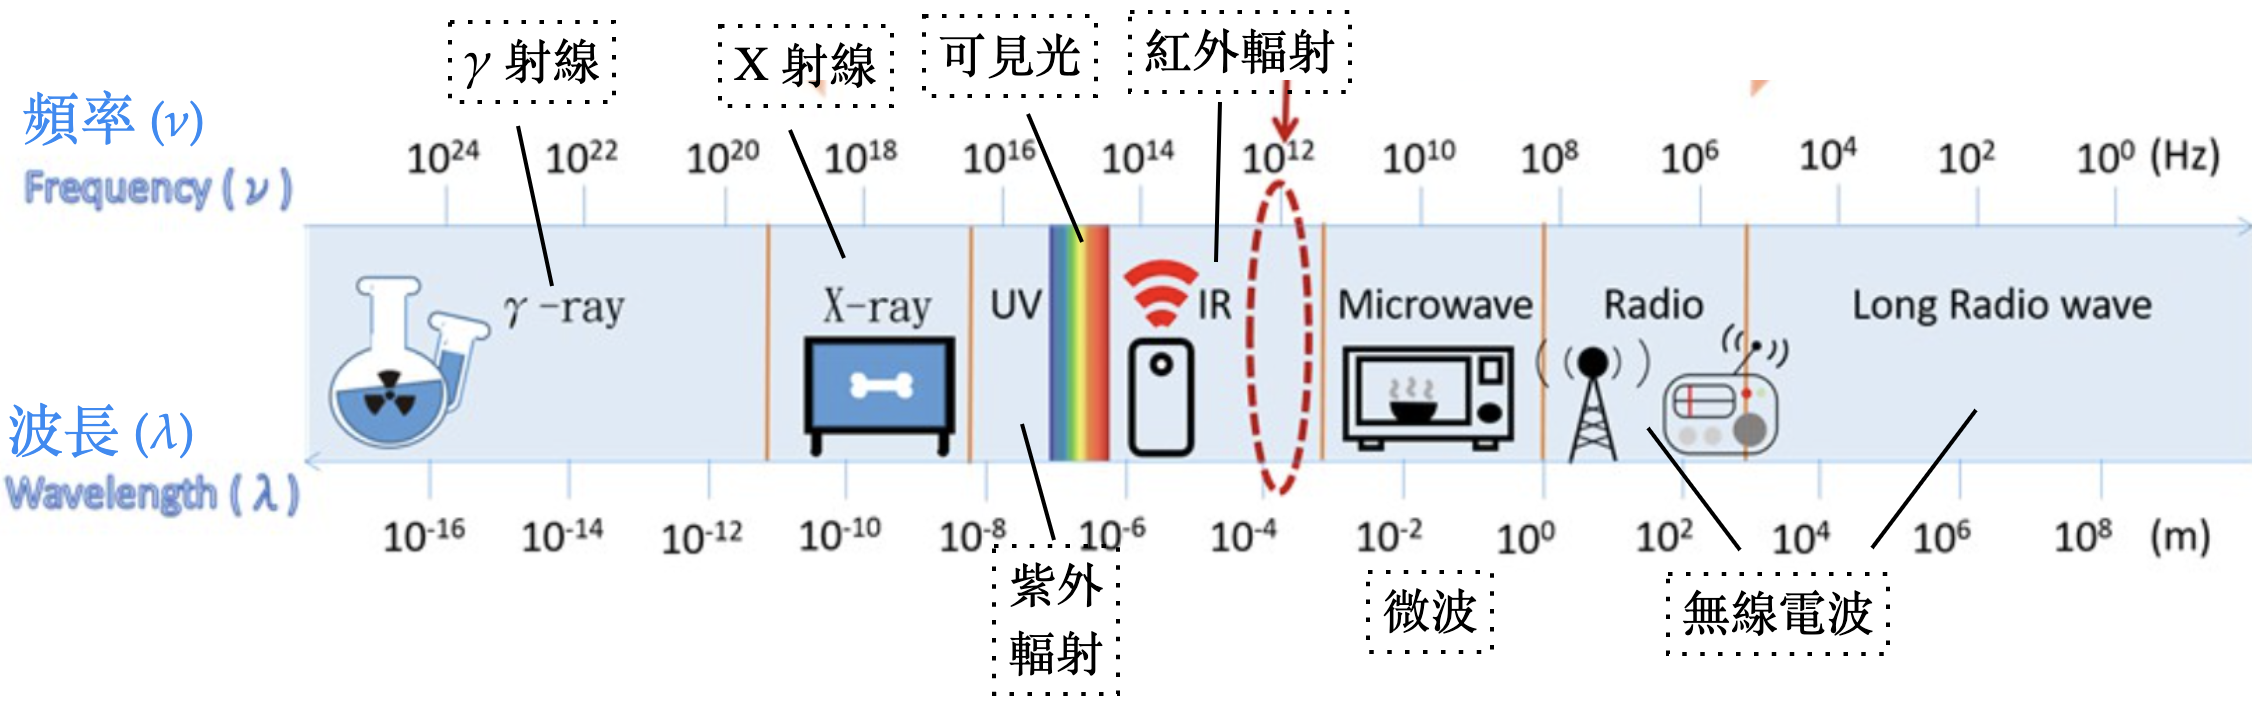
\includegraphics[width=\textwidth]{./img/ch1_2024-05-06-18-34-04.png}\par}
    \par{\par\centering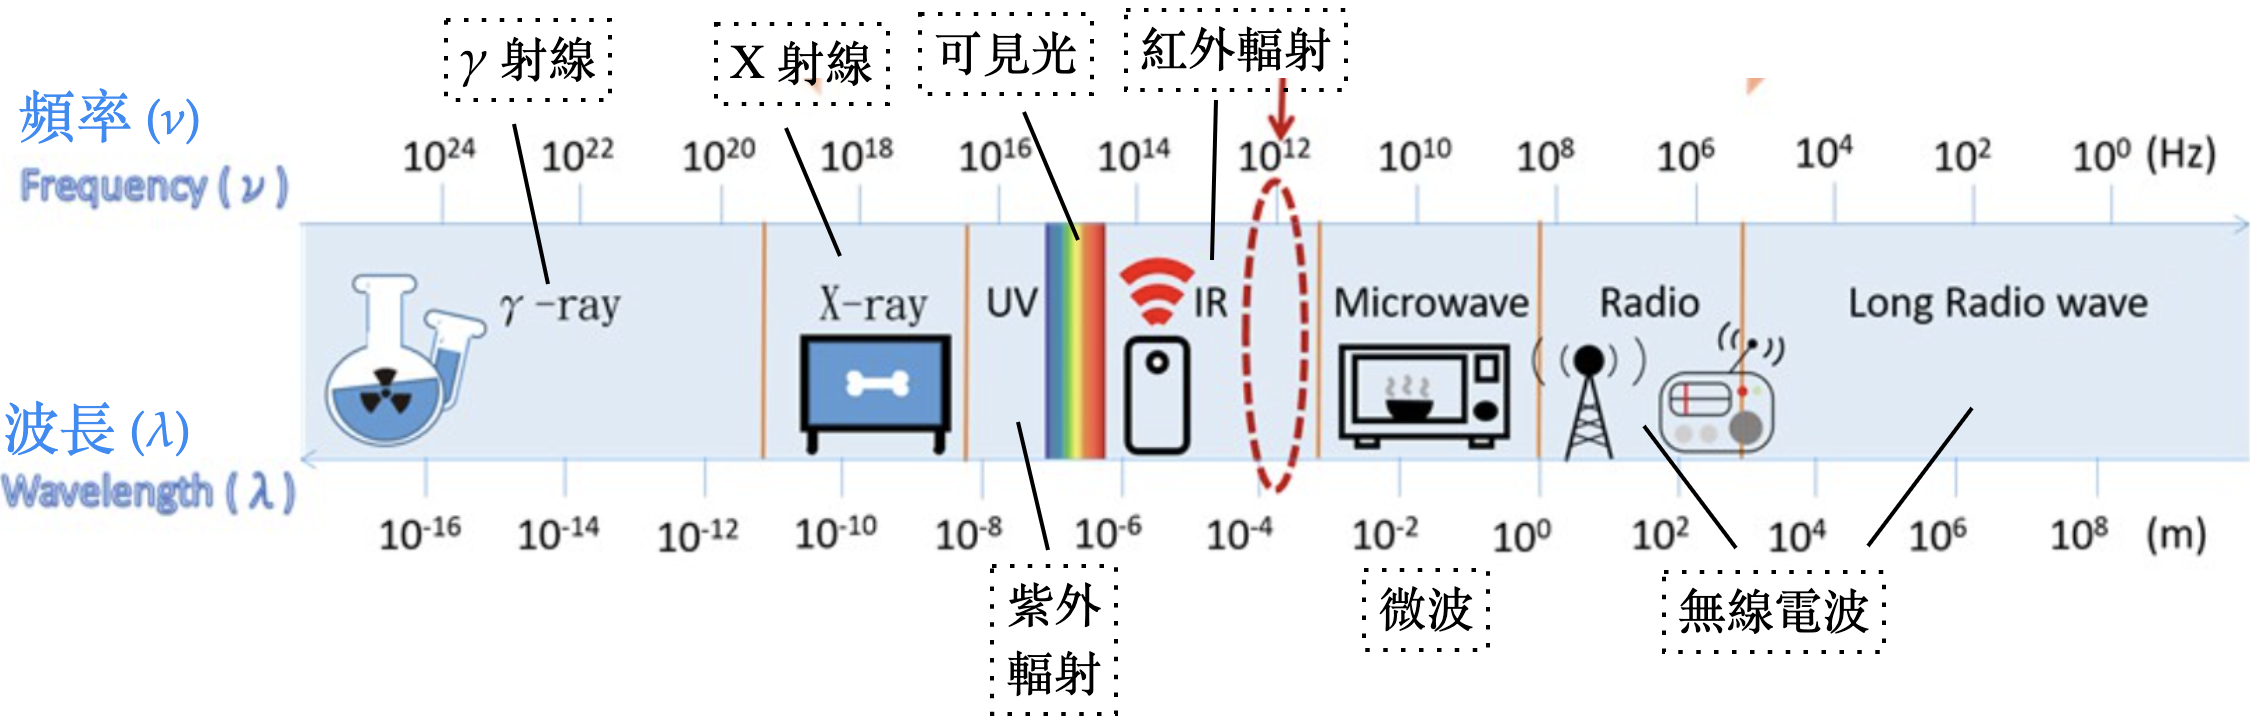
\includegraphics[width=\textwidth]{./img/ch1_2024-05-06-18-39-52.png}\par}
\end{frame}

\begin{frame}{電磁波的性質 Properties of electromagetic wave}
    \begin{itemize}
        \item 電磁波是由振動的電場及磁場組成。\\Electromagnetic wave is formed by oscillating electric and magnetic fields.
        \item 電磁波可以在真空中傳播,機械波則不能。\\Electromagnetic waves can travel in vacuum while mechanical wave cannot.
        \item 電磁波只能是橫波。\\Electromagnetic wave can only be transverse wave.
        \item 在電場或磁場下,所有電磁波都不會偏轉其傳播方向。\\Neither electric or magnetic fields can deflect a EM wave.
    \end{itemize}
\end{frame}

\section{discribing wave}

\begin{frame}
    \frametitle{描述波Describing waves}
    \par{\par\centering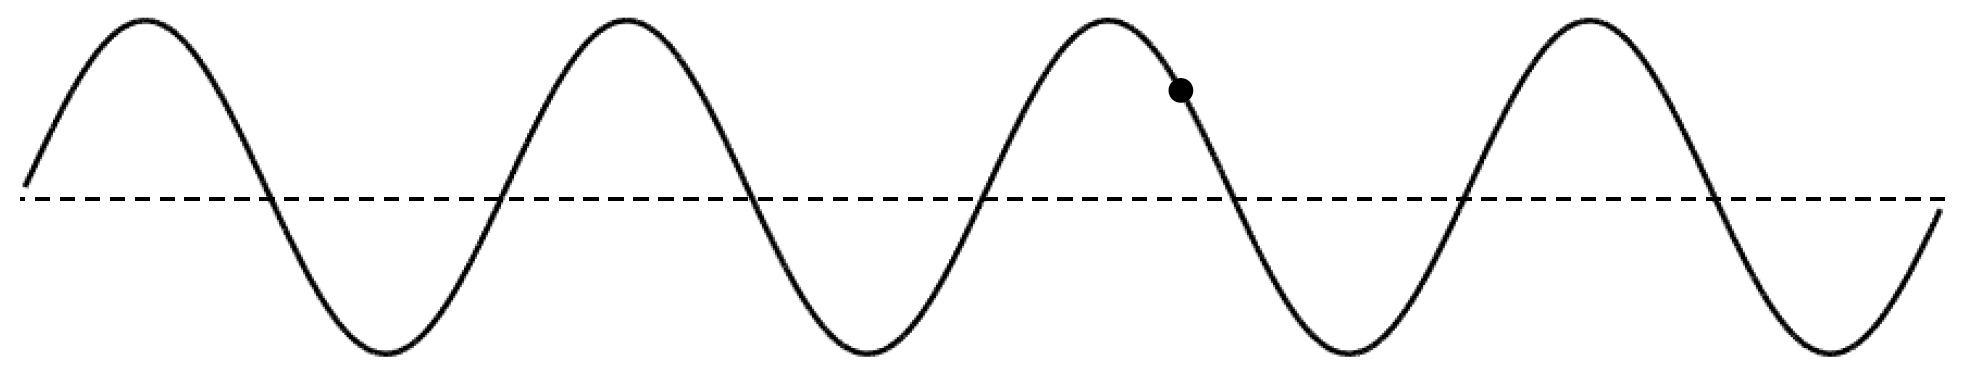
\includegraphics[width=.75\textwidth]{./img/ch1_2024-05-06-20-43-46.png}\par}
    % \begin{itemize}
    %     \item 平衡位置:假設沒有波,質點應該所在的位置。\\Equilibrium position: the position where the particle would naturally rest in the absence of wave.
    %     \item 位移:質點從其平衡位置至現時位置的距離和方向。\\Displacement: distance and direction of a particle from equilibrium position to current position.
    %           \begin{itemize}
    %               \item 位移是一個矢量。\\Displacement is a vector.
    %           \end{itemize}
    % \end{itemize}
    \begin{block}{平衡位置Equilibrium position}
        假設沒有波,質點應該所在的位置。\\The position where the particle would naturally rest in the absence of wave.
    \end{block}
    \begin{block}{位移Displacement ($y$)}
        \begin{itemize}
            \item 質點從其平衡位置至現時位置的距離和方向。\\distance and direction of a particle from equilibrium position to current position.
            \item 位移是一個向量。
        \end{itemize}
    \end{block}
\end{frame}


\begin{frame}
    \frametitle{描述波Describing waves}
    \par{\par\centering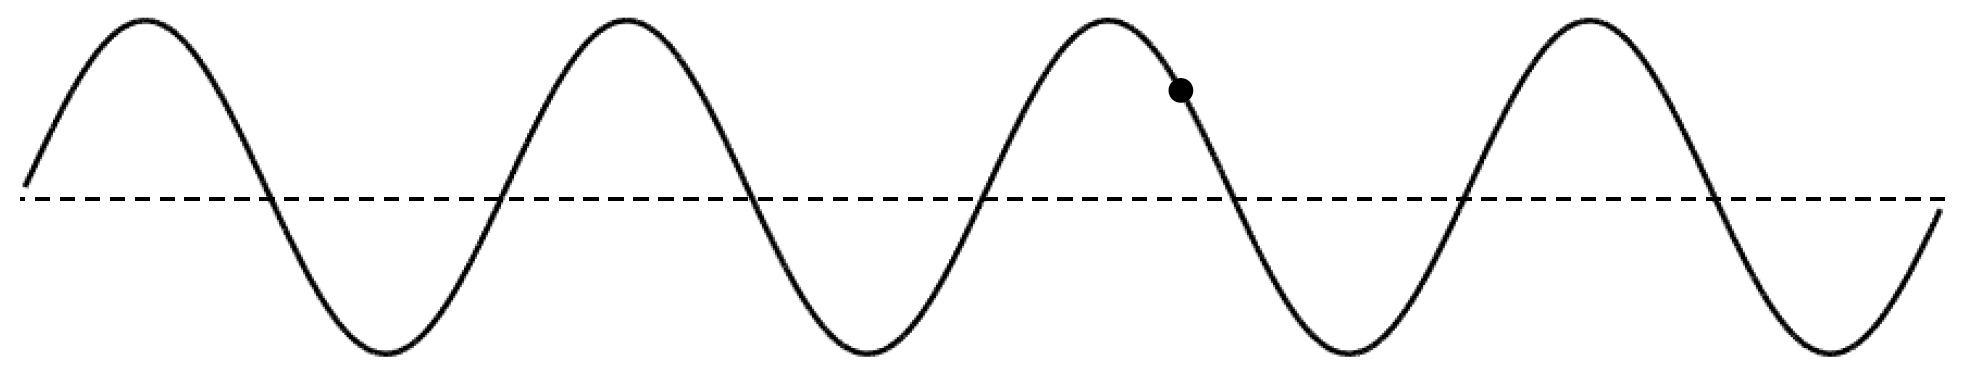
\includegraphics[width=.75\textwidth]{./img/ch1_2024-05-06-20-43-46.png}\par}
    \begin{block}{振幅Amplitude ($A$)}
        \begin{itemize}
            \item 質點離平衡位置的\textbf{最大位移}。\\The maximum displacement from equilibrium position.
            \item 振幅和波的質點的機械能有關。\\Amplitude is related the mechanical energy of a particle in a wave.
                  \begin{itemize}
                      \item 振幅較大的波盛載較多的能量。\\Greater amplitude means greater mechanical energy.
                  \end{itemize}
        \end{itemize}
    \end{block}
\end{frame}

\begin{frame}
    \frametitle{波長Wavelength $\lambda$}

    \par{\par\centering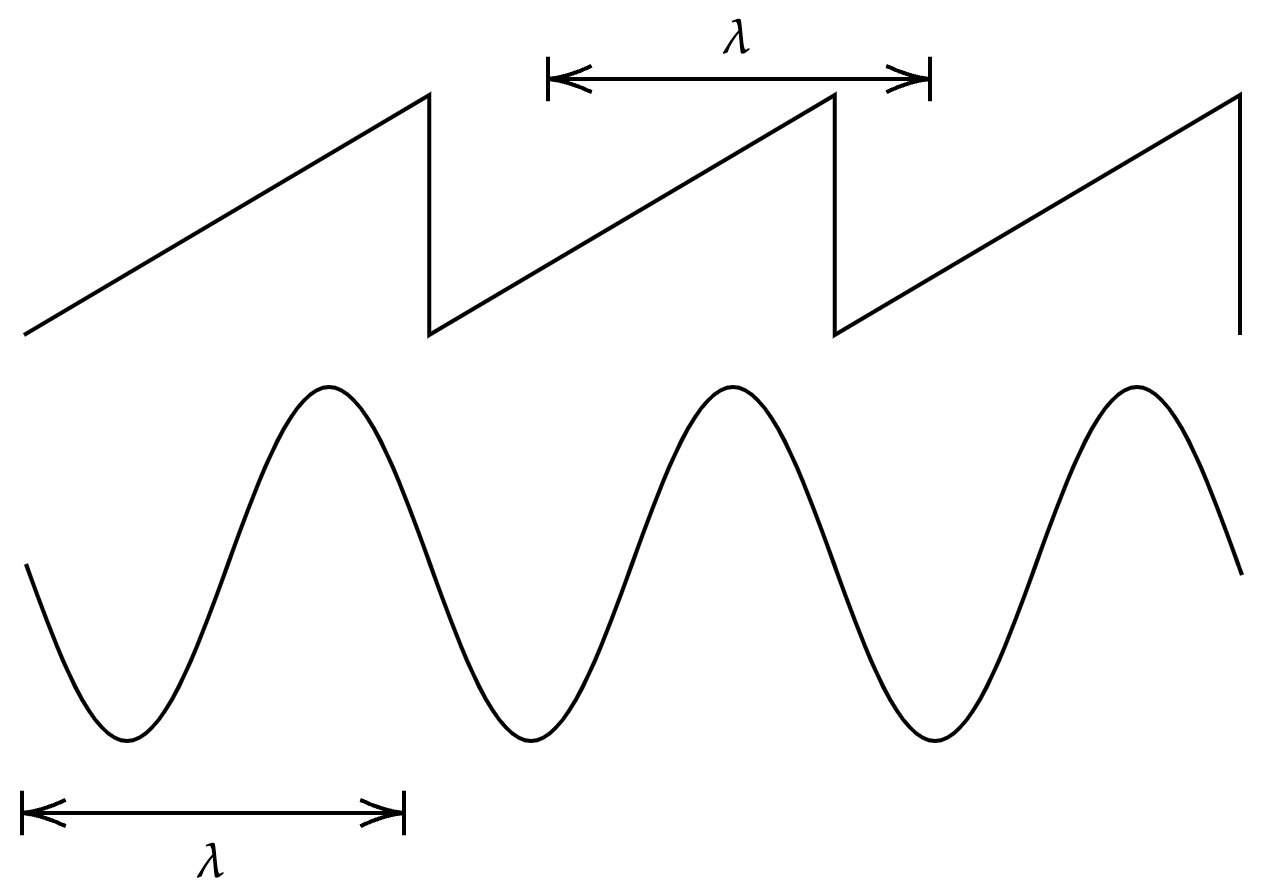
\includegraphics[width=.6\textwidth]{./img/ch1_2024-05-06-21-13-45.png}\par}

    \begin{itemize}
        \item 波長是一個質點完成一個完整振動時,波行走距離。
    \end{itemize}
\end{frame}

\begin{frame}
    \frametitle{波長Wavelength $\lambda$}

    % \par{\par\centering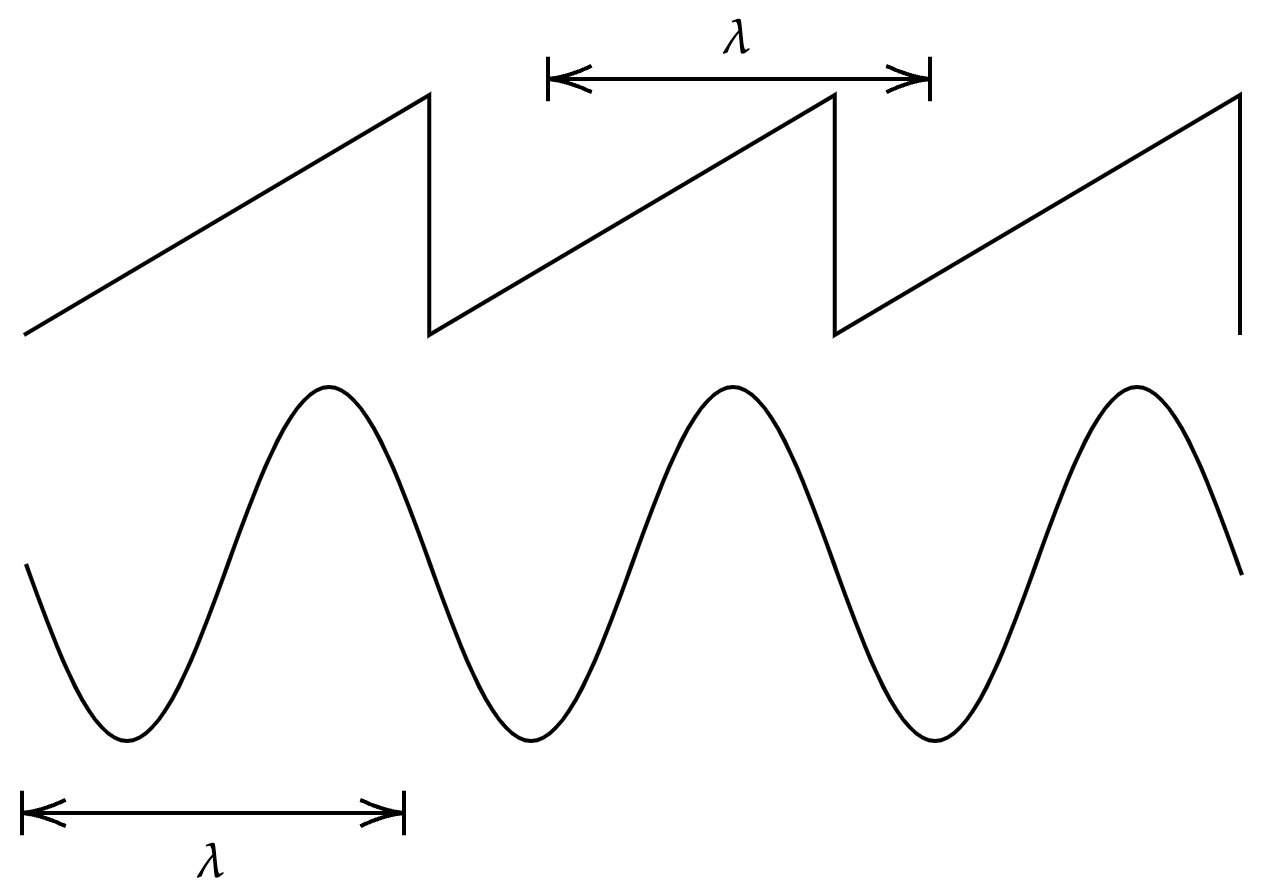
\includegraphics[width=.6\textwidth]{./img/ch1_2024-05-06-21-13-45.png}\par}
    \begin{itemize}
        \item 也是波重複自身形狀的最短距離。
        \item 也是兩個同相的點之間的最短距離。
        \item 單位Unit: [m]
    \end{itemize}
\end{frame}

\begin{frame}
    \frametitle{週期Period $T$}
    \begin{itemize}
        \item 波的週期$T$是每個質點完成一個完整振動所需的時間。
        \item 單位Unit: [s]
    \end{itemize}
    % \par{\par\centering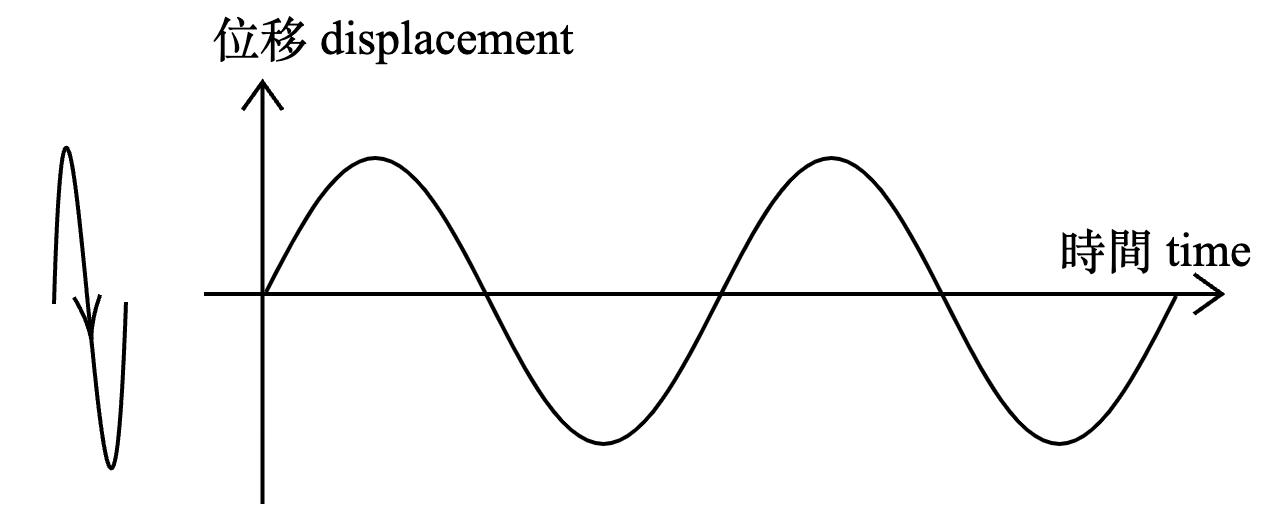
\includegraphics[width=.7\textwidth]{./img/ch1_2024-05-06-21-34-22.png}\par}
    \bigskip\par{\par\centering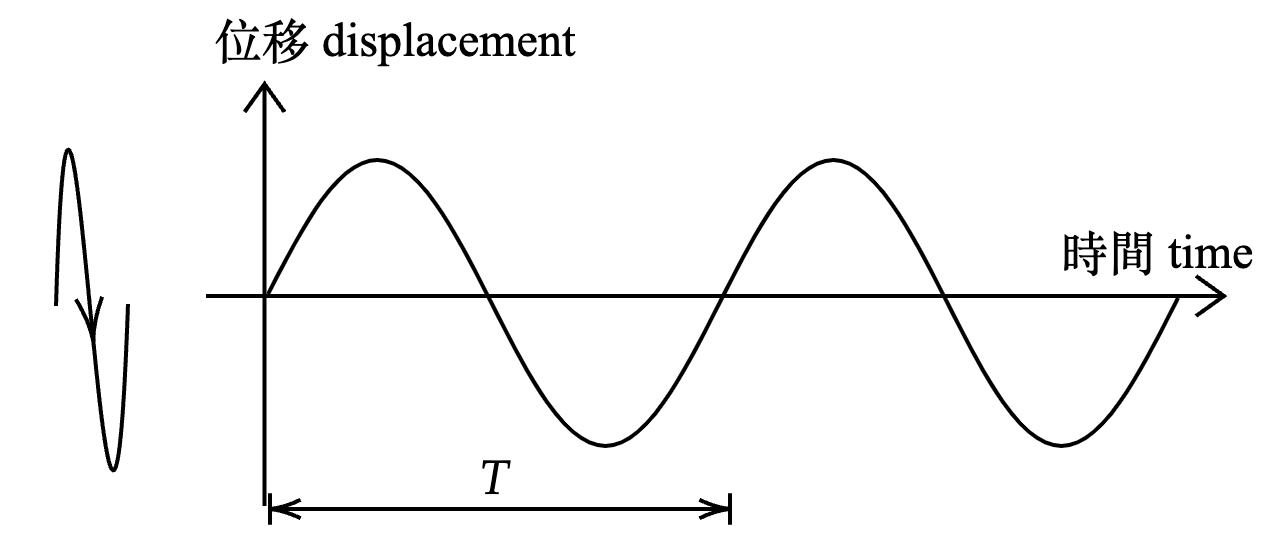
\includegraphics[width=.7\textwidth]{./img/ch1_2024-05-07-18-12-56.png}\par}
\end{frame}

\begin{frame}
    \frametitle{週期Period $T$}

    \begin{itemize}
        \item 週期 $T$ 也是一個行波傳播一個波長距離所需的時間。
    \end{itemize}
    \par{\par\centering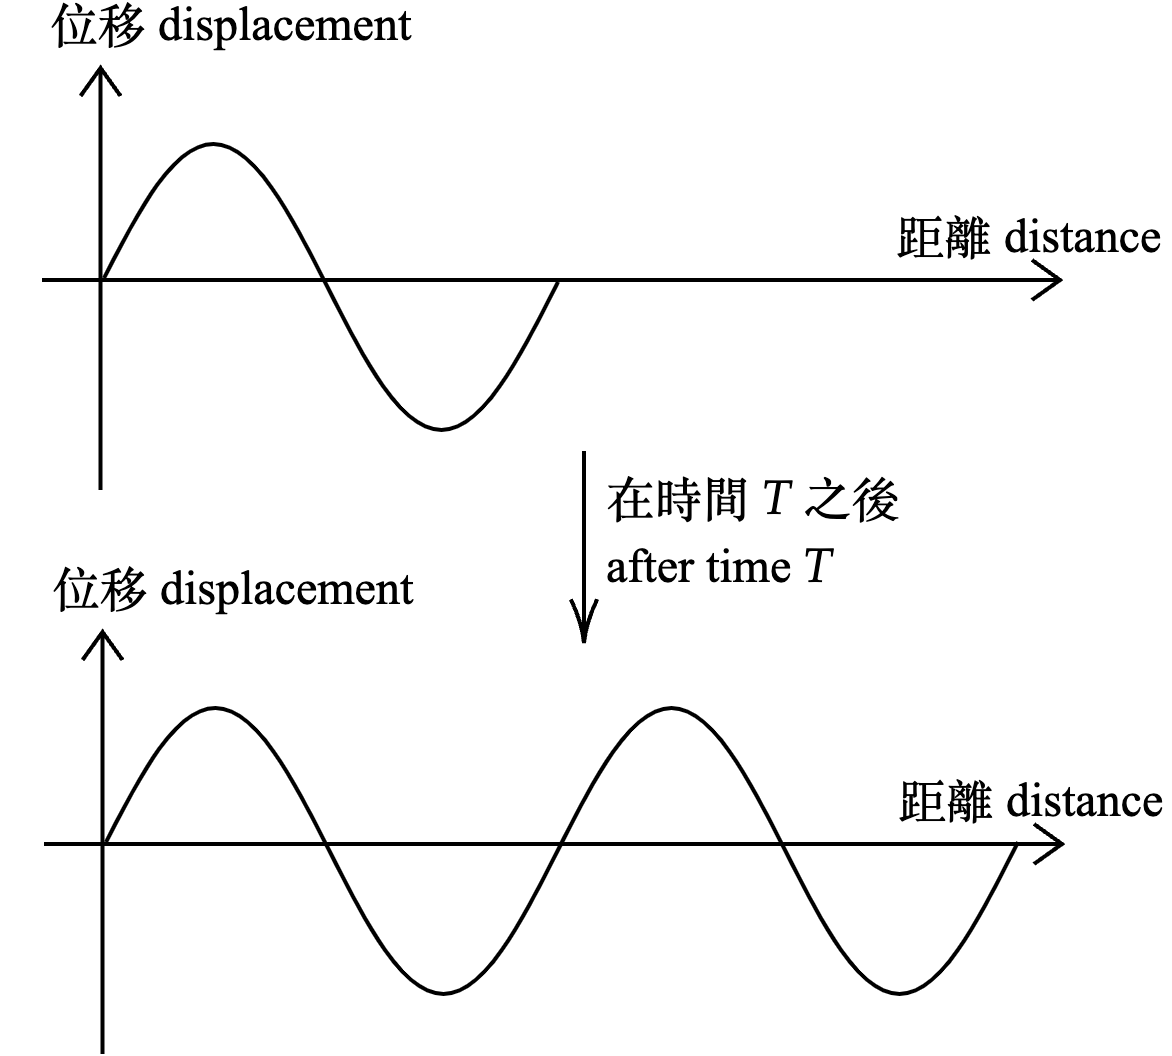
\includegraphics[width=.6\textwidth]{./img/ch1_2024-05-07-18-16-42.png}\par}
\end{frame}

\begin{frame}
    \frametitle{頻率Frequency $f$}
    \begin{itemize}
        \item 頻率 $f$ 是質點在一秒內完成多少次循環。
        \item 或是一秒內有多少個完整的波經過某點。
        \item 單位Unit: [Hz]
    \end{itemize}
    \par{\par\centering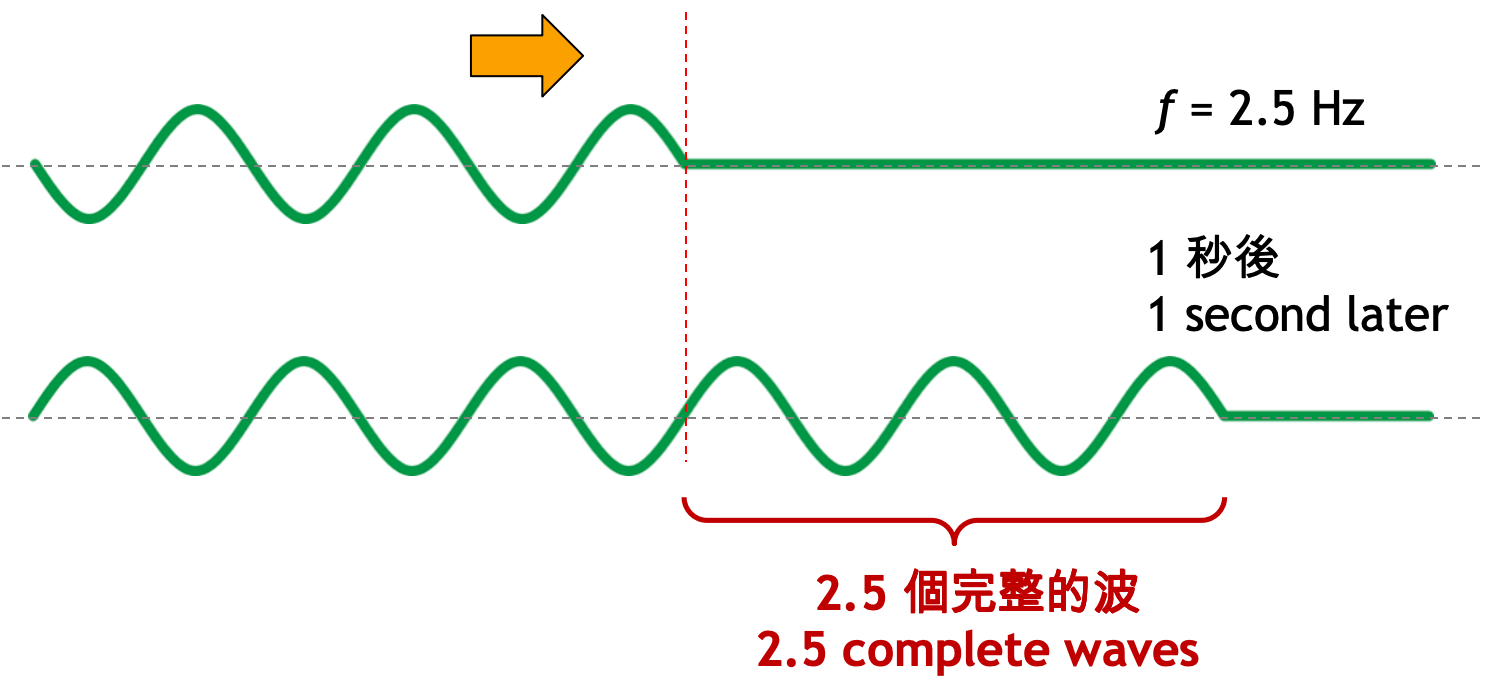
\includegraphics[width=.75\textwidth]{./img/ch1_2024-05-08-15-21-40.png}\par}
\end{frame}

\begin{frame}{頻率Frequency $f$}
    \begin{itemize}
        \item 在同一個連續波中,所有質點必須具有相同的頻率。
        \item 頻率的大小僅取決於\textbf{波源}。
    \end{itemize}\bigskip
    \begin{alertblock}{頻率和週期的關係Relationship between frequency and period}
        \[f=\frac{1}{T}\]
    \end{alertblock}
\end{frame}

\begin{frame}
    \frametitle{波速 speed of wave $v$}
    一列波在每單位時間內的傳播距離。
    \par{\par\centering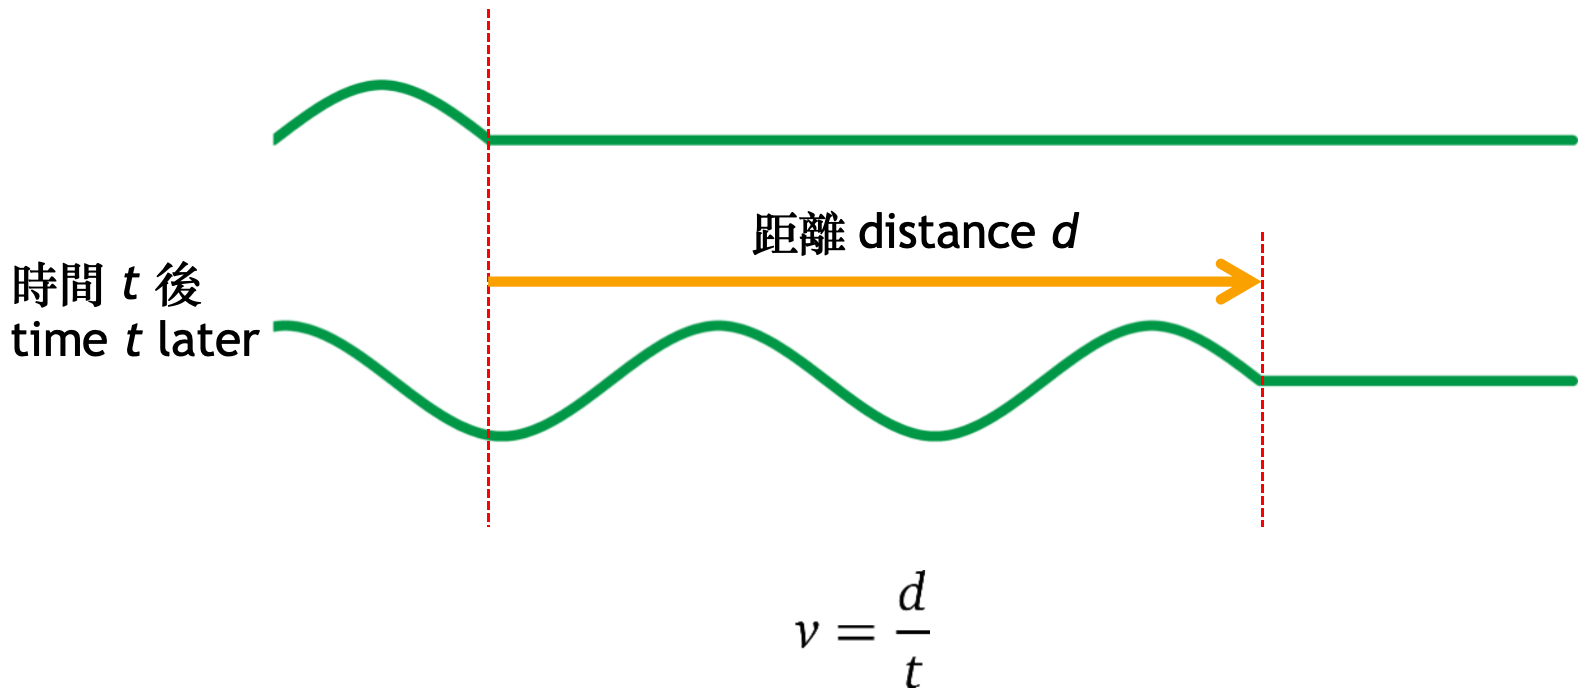
\includegraphics[width=\textwidth]{./img/ch1_2024-05-08-15-14-23.png}\par}
\end{frame}

\begin{frame}{波速v}
    \begin{itemize}
        \item 對於行波來說:
    \end{itemize}\bigskip
    % \input{nodes}
    % \par{\par\centering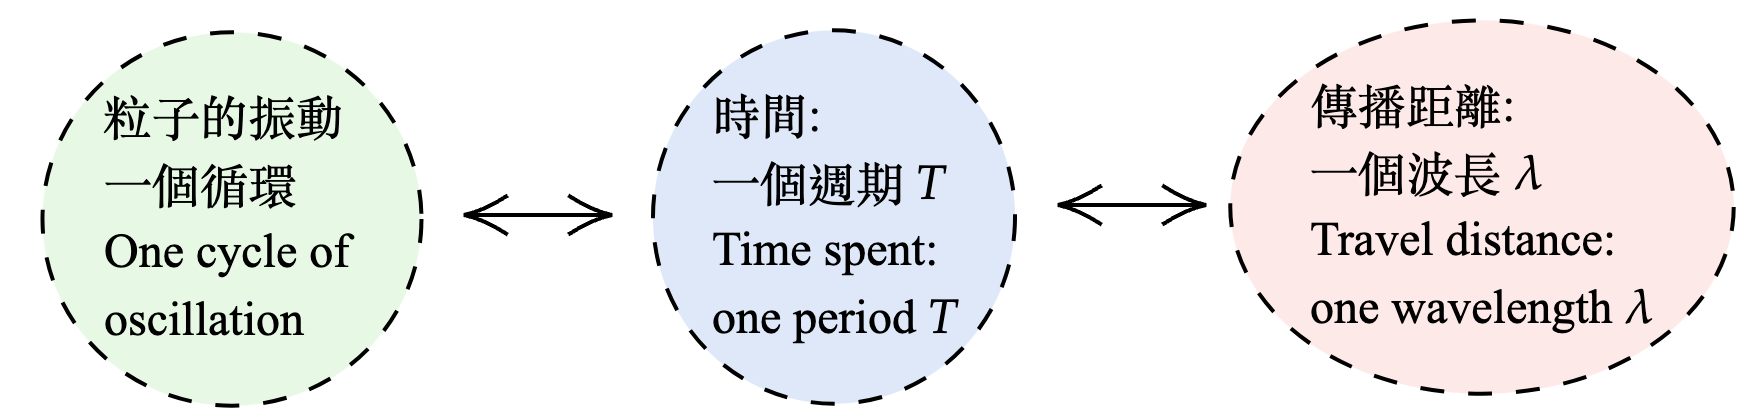
\includegraphics[width=\textwidth]{./img/ch1_2024-05-08-15-48-22.png}\par}
    \par{\par\centering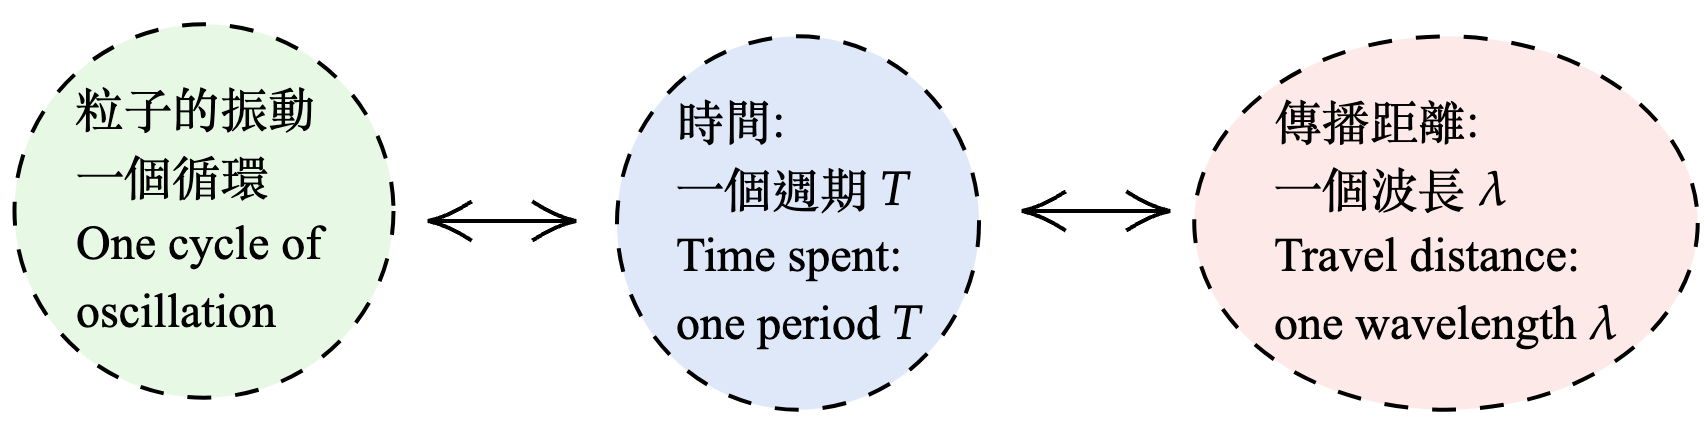
\includegraphics[width=\textwidth]{./img/ch1_2024-05-08-15-56-03.png}\par}
    % \bigskip

    \begin{alertblock}{波動方程式}
        \begin{align*}
            v & =\frac{\lambda}{T} \\
            v & =f\,\lambda
        \end{align*}
    \end{alertblock}
\end{frame}

\begin{frame}[t]{例題Example}
    \par{\par\centering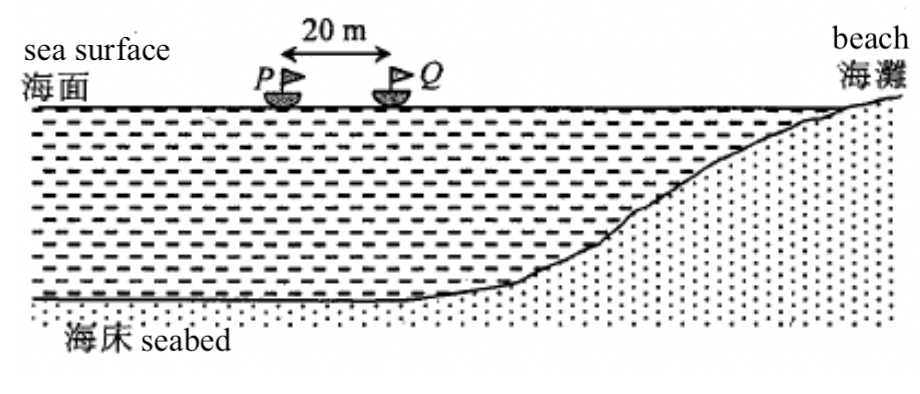
\includegraphics[width=.5\textwidth]{./img/ch1_2024-05-09-14-34-58.png}\par}
    圖中顯示某海灘的切面圖及兩隻小船所在的位置。$PQ= \qty{20}{m}$。現有平
    直的波浪向着海灘前進。波浪從 $P$ 運行至 $Q$ 需時 \qty{4}{s}。求波浪在 $P$、$Q$
    之間運行時的平均速率。
\end{frame}

\begin{frame}[t]{例題Example}
    下圖是相同的繩子在不同時間的情況,求最大的週期和波動對應的移動
    方向。
    \bigskip
    \par{\par\centering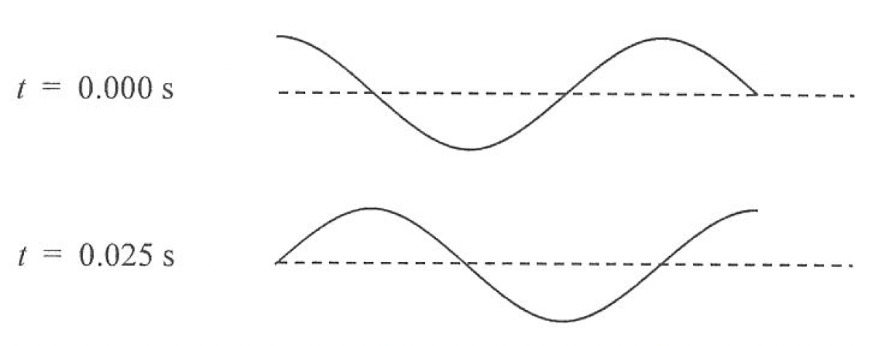
\includegraphics[width=.7\textwidth]{./img/ch1_2024-05-08-16-37-34.png}\par}
\end{frame}

% rejected because it's a y-t graph
\begin{frame}[t]{例題Example}
    圖中是一個質點在行波中的位移-時間圖。求波的頻率。
    \par{\par\centering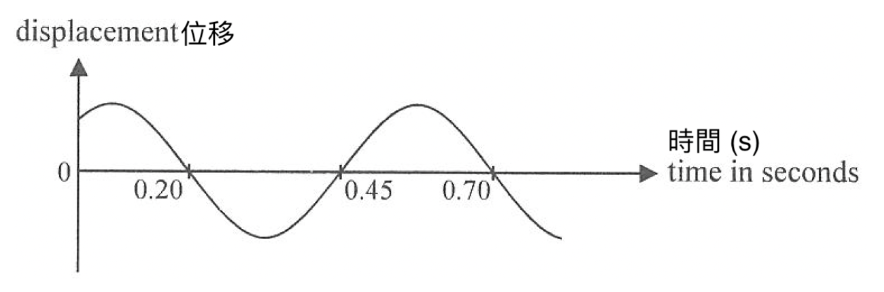
\includegraphics[width=.66\textwidth]{./img/ch1_2024-05-08-16-40-38.png}\par}
\end{frame}

\begin{frame}[t]{例題Example}
    % \par{\par\centering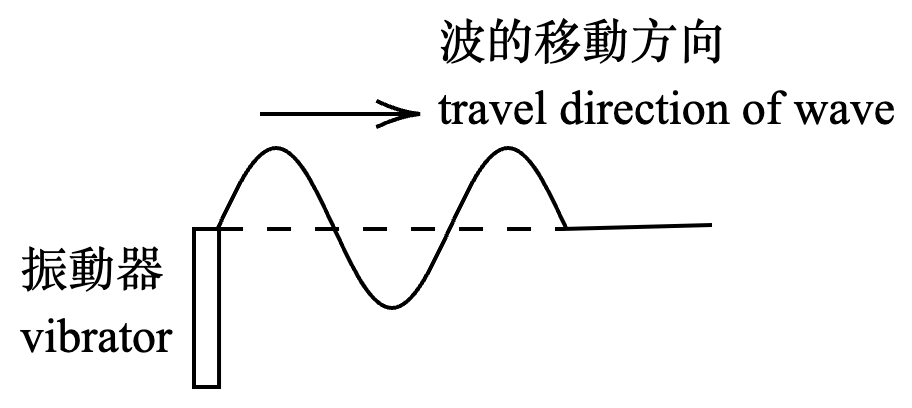
\includegraphics[width=.3\textwidth]{./img/ch1_2024-05-08-17-23-14.png}\par}
    \par{\par\centering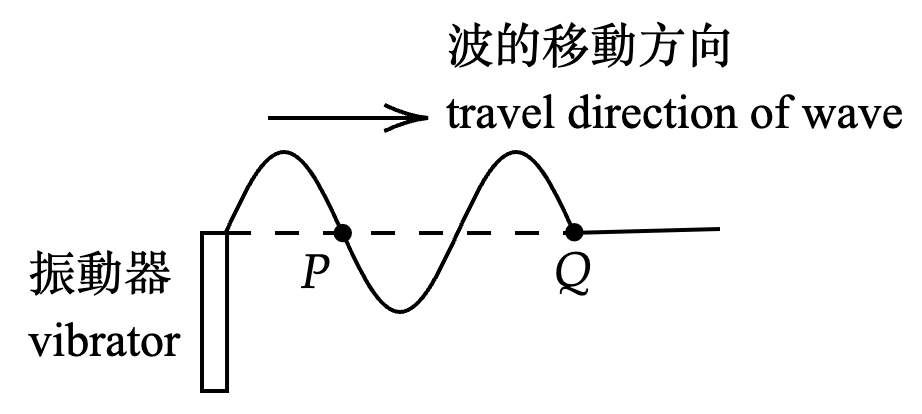
\includegraphics[width=.5\textwidth]{./img/ch1_2024-05-08-17-25-50.png}\par}\bigskip
    一振動器在一根繩上產生行波。上圖顯示該繩在某瞬間的形狀。下列各圖中,那個顯示在四分之一週期後,$P$和$Q$之間該繩的形狀?
\end{frame}

\begin{frame}[t]{例題Example}
    \begin{tasks}[label-offset=.6em,item-indent=2em](2)
        \task \topalign{\par\centering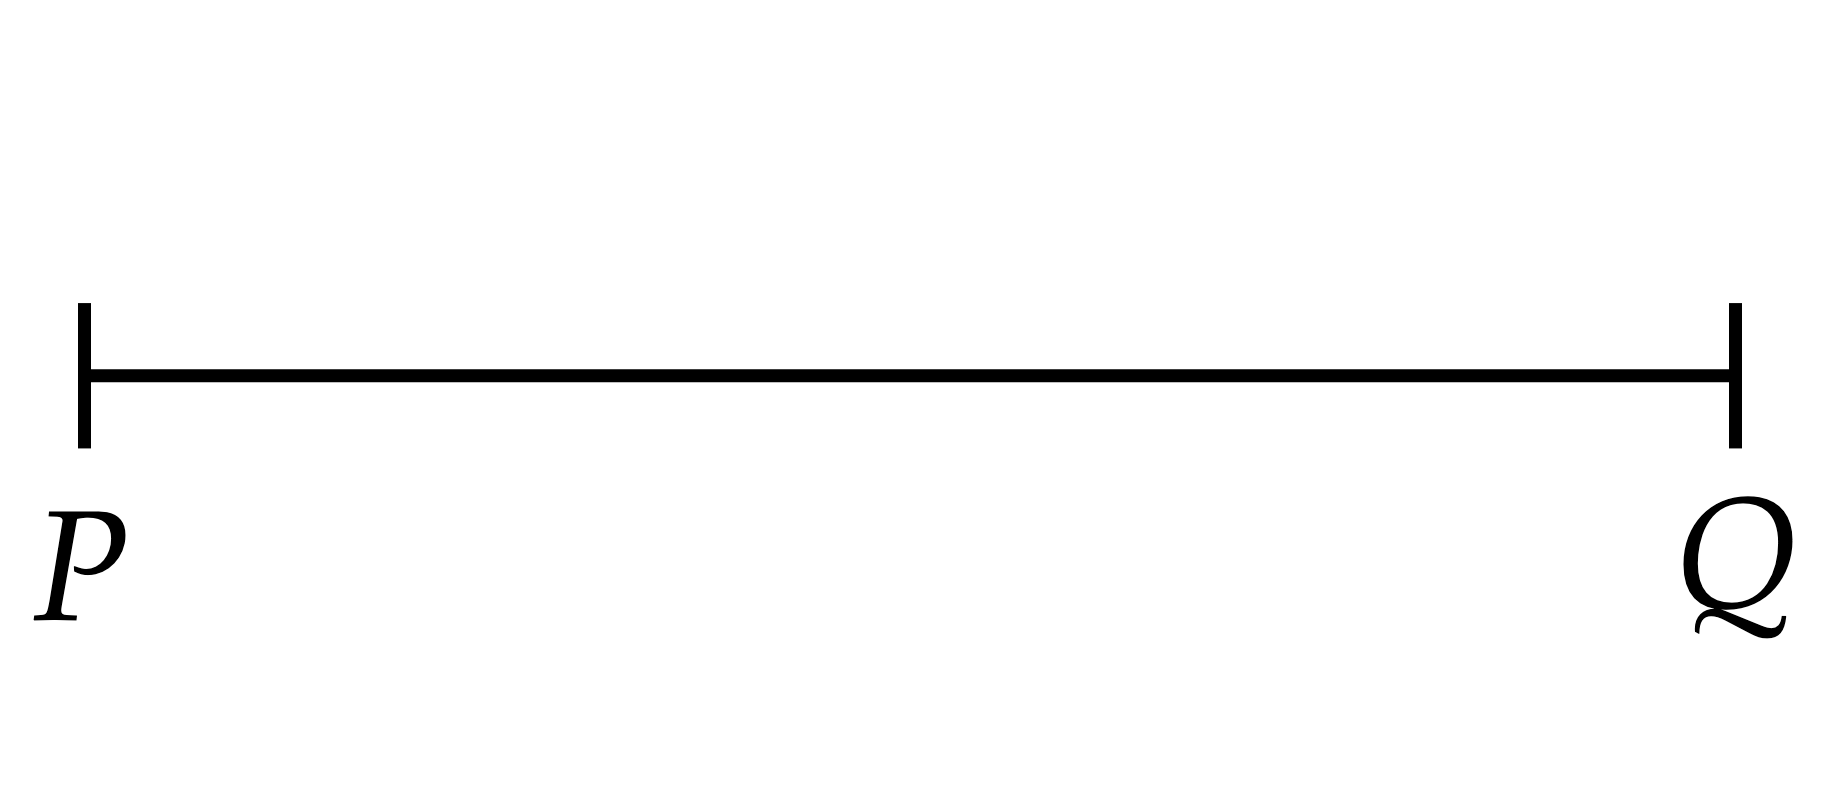
\includegraphics[width=.4\textwidth]{./img/ch1_2024-05-08-17-29-34.png}\par}
        \task \topalign{\par\centering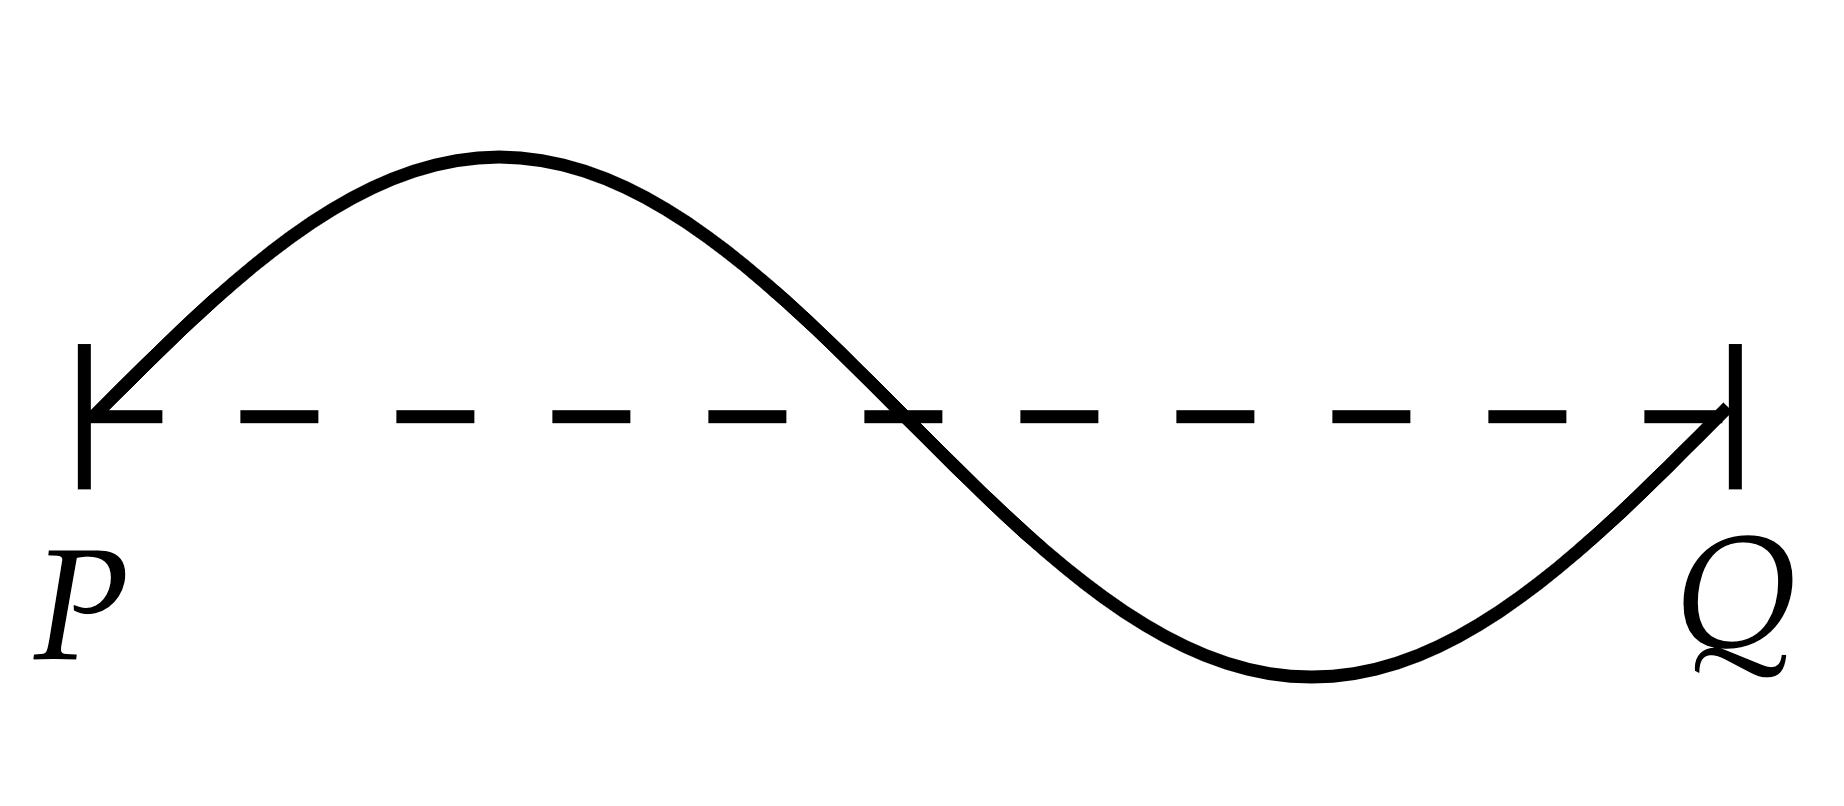
\includegraphics[width=.4\textwidth]{./img/ch1_2024-05-08-17-33-59.png}\par}
        \task \topalign{\par\centering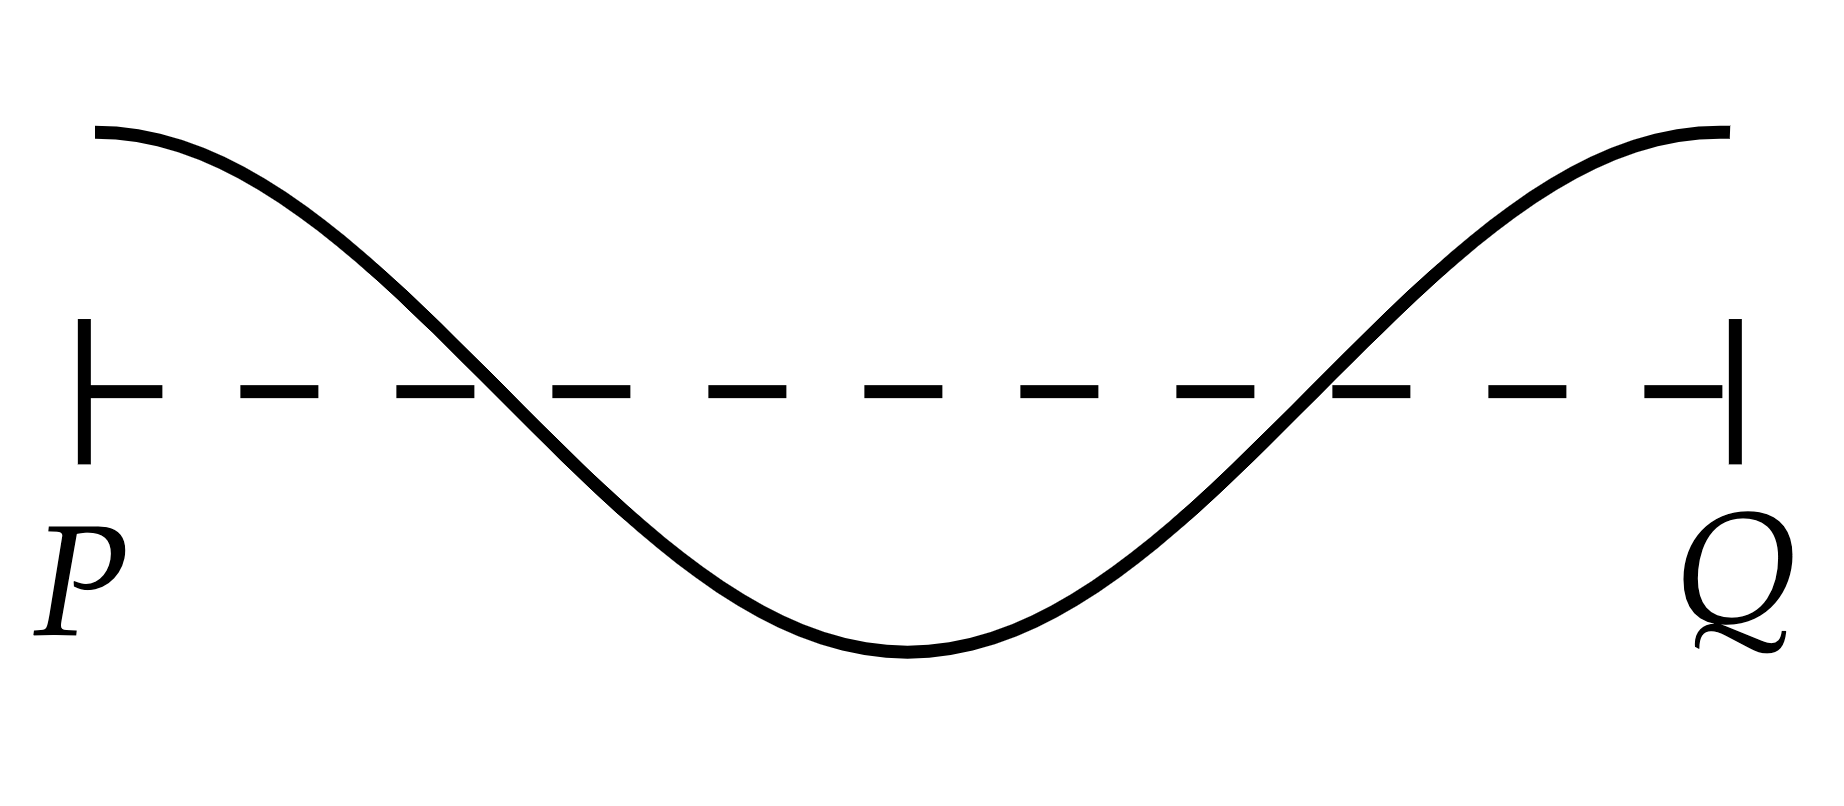
\includegraphics[width=.4\textwidth]{./img/ch1_2024-05-08-17-35-34.png}\par}
        \task \topalign{\par\centering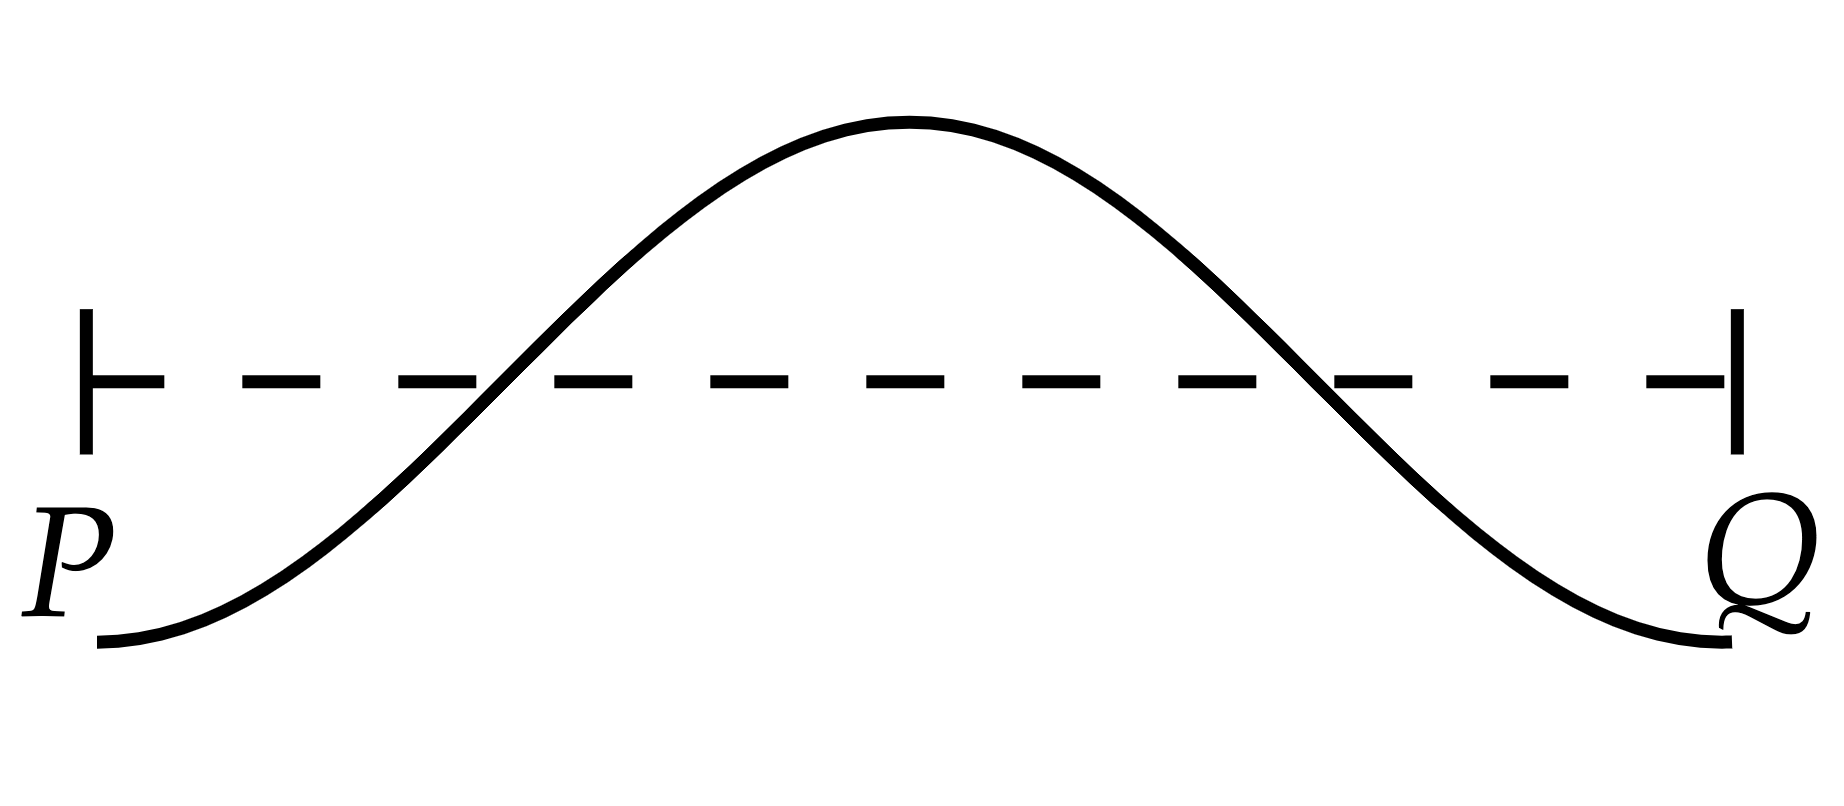
\includegraphics[width=.4\textwidth]{./img/ch1_2024-05-08-17-35-56.png}\par}
    \end{tasks}
\end{frame}

\begin{frame}[t]{例題Example}
    當一列水波經過一枚放在水中的木塞時,木塞在 \qty{2}{s} 內上下振動了四次。水波兩個相鄰波峰之間的距離為 \qty{10}{cm}。求水波的速率。
\end{frame}

\begin{frame}[t]{例題Example}
    一個水槽中盛有水,一個振動器在水面振動。它設定成每秒振動 20 次。
    \begin{itemize}
        \item [(a)] 求它產生的水波的週期。
    \end{itemize}
\end{frame}

\begin{frame}[t]{例題Example}
    \begin{itemize}
        \item [(b)] 若水波的波速是 \qty{32}{cm.s^{-1}},求水波的波長。
    \end{itemize}
\end{frame}

\begin{frame}[t]{例題Example}
    \begin{itemize}
        \item [(c)] 寫出兩個方法增加水波波長。
    \end{itemize}
\end{frame}




\begin{frame}
    \frametitle{波速 speed of wave $v$}
    \begin{itemize}
        \item 波的速度取決於波所傳播的\textbf{介質}。
        \item 例如:光波在空氣、水和玻璃中會以不同的速度傳播。
    \end{itemize}
    \bigskip \bigskip
    \textbf{影響波速的因素:\\Factor affecting speed of wave:}
    \begin{exampleblock}{水波 Water wave}
        深水快,淺水慢。
    \end{exampleblock}

\end{frame}

\begin{frame}{影響波速的因素Factor affecting speed of wave}

    \begin{exampleblock}{繩子上的橫波 Transverse wave on a rope}
        \begin{itemize}
            \setlength{\itemsep}{.6em}
            \item $\displaystyle v=\sqrt{\frac{T}{\mu}} $
            \item 張力Tension T $\uparrow \;\rightarrow$ 波速speed $\uparrow$。
            \item 繩子每米的質量Mass per unit length $\mu\uparrow \;\rightarrow$波速speed$\downarrow$。
        \end{itemize}
    \end{exampleblock}
    \begin{exampleblock}{聲波Sound wave}
        波速比較Speed comparison:$v_{\texttt{ 固體solid}}>v_{\texttt{ 液體liquid}}>v_{\texttt{ 氣體gas}}$。
    \end{exampleblock}

    \begin{exampleblock}{電磁波Electromagnetic wave}
        折射率Refractive index n $\uparrow \;\rightarrow$ 波速speed $\downarrow$。
    \end{exampleblock}
\end{frame}

\begin{frame}
    \frametitle{波峰和波谷Crest and trough}
    \par{\par\centering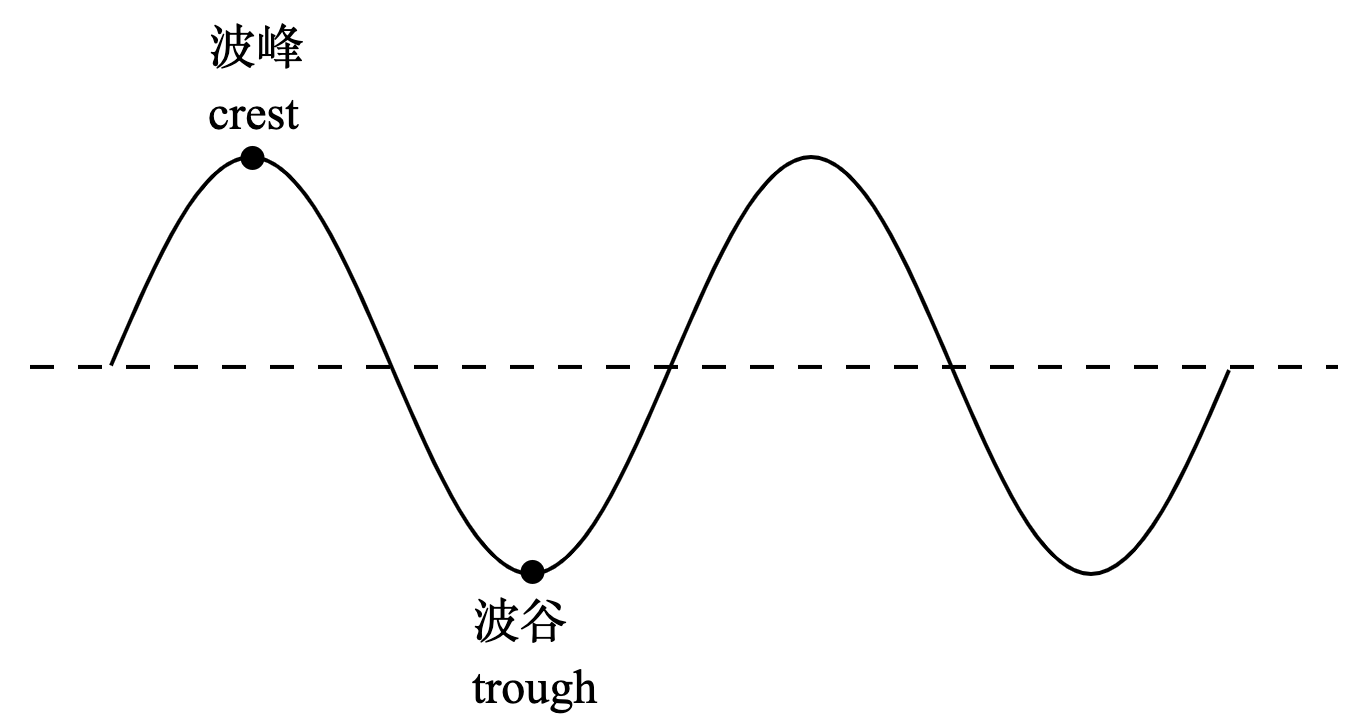
\includegraphics[width=.7\textwidth]{./img/ch1_2024-05-09-11-41-18.png}\par}
    \begin{itemize}
        \item 波峰(波谷)和相鄰波峰(波谷)之間的距離等於一個波長 $\lambda$。
        \item 若質點在波峰或波谷上,位移的量值等於振幅 $A$。
        \item 波峰或波谷上的質點必定是瞬時靜止。
    \end{itemize}
\end{frame}

\begin{frame}
    \frametitle{密部中心和疏部中心Compression centre and rarefraction centre}
    \bigskip
    \par{\par\centering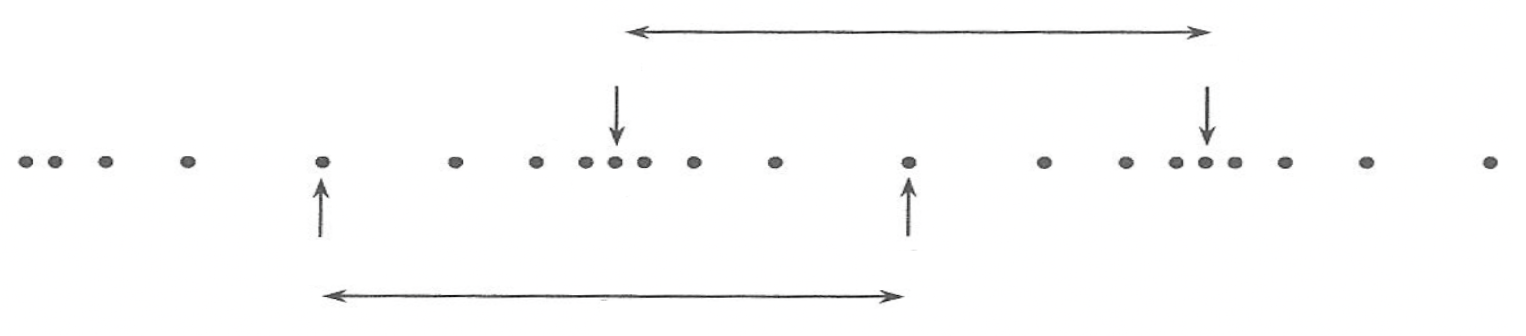
\includegraphics[width=.8\textwidth]{./img/ch1_2024-05-09-11-45-52.png}\par}
    \bigskip \bigskip

    \begin{itemize}
        \item 質點在密部和疏部時,其處於平衡位置。
        \item 密部(疏部)和相鄰密部(疏部)之間的距離等於一個波長 $\lambda$。

    \end{itemize}
\end{frame}





\begin{frame}
    \frametitle{密部中心和疏部中心Compression centre and rarefraction centre}
    \begin{itemize}
        \item 密部和疏部上的質點速率為最大值。
        \item 密部(疏部)和相鄰密部(疏部)中間的質點處於極端位置,其位
              移等於振幅。
    \end{itemize}
\end{frame}

\begin{frame}{關係線圖Displacement relation graphs}
    \begin{block}{位移-距離圖displacement-distance graph}
        表示一瞬間各個質點的位移情況。
    \end{block}\bigskip
    \begin{block}{位移-時間圖displacement-time graph}
        表示一個質點在不同時間段的位移情況。
    \end{block}
\end{frame}


\begin{frame}
    \frametitle{行波和位移-距離圖Travelling wave and displacement-distance graph}
    % Given the movement direction of wave,
    % \par{\par\centering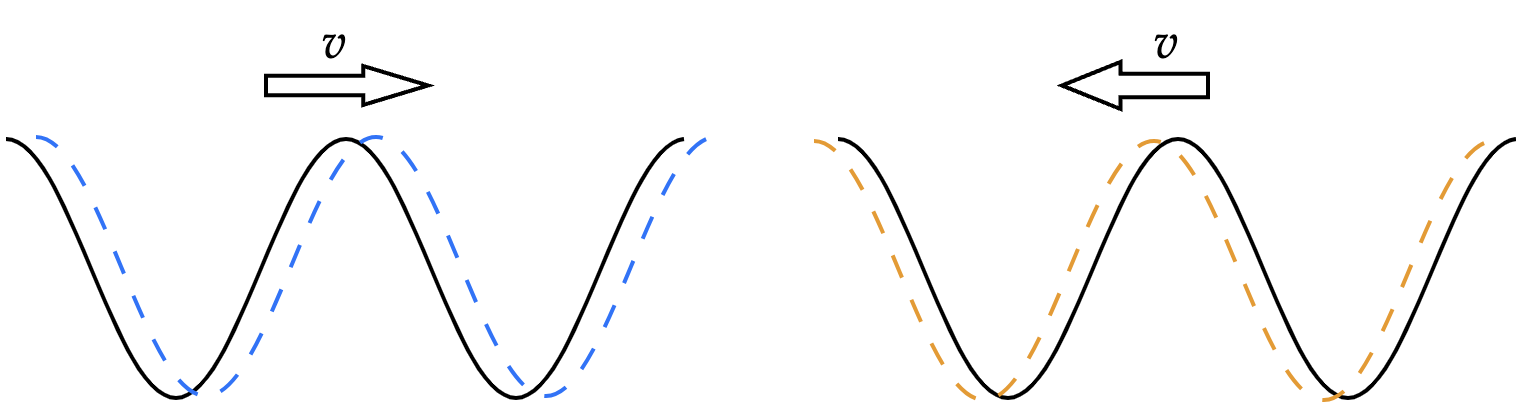
\includegraphics[width=\textwidth]{./img/ch1_2024-05-09-14-44-12.png}\par}
    % \par{\par\centering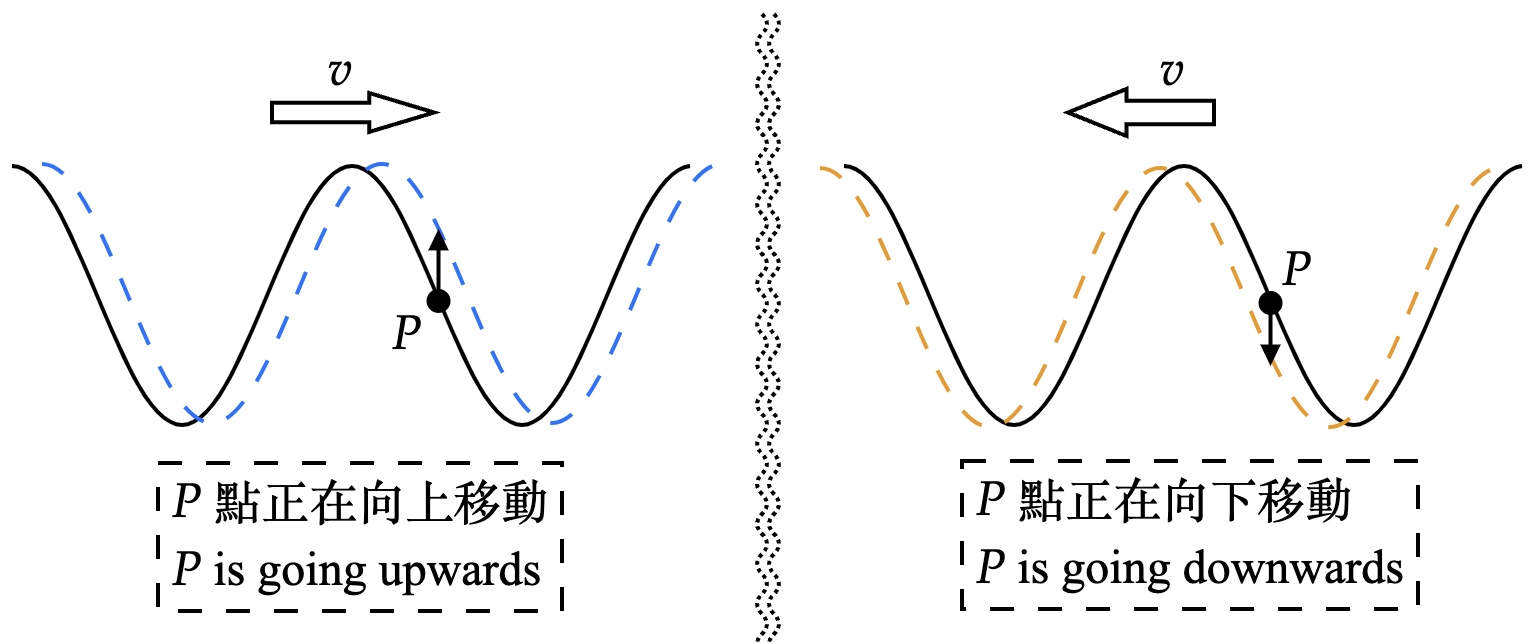
\includegraphics[width=\textwidth]{./img/ch1_2024-05-09-14-57-13.png}\par}
    \par{\par\centering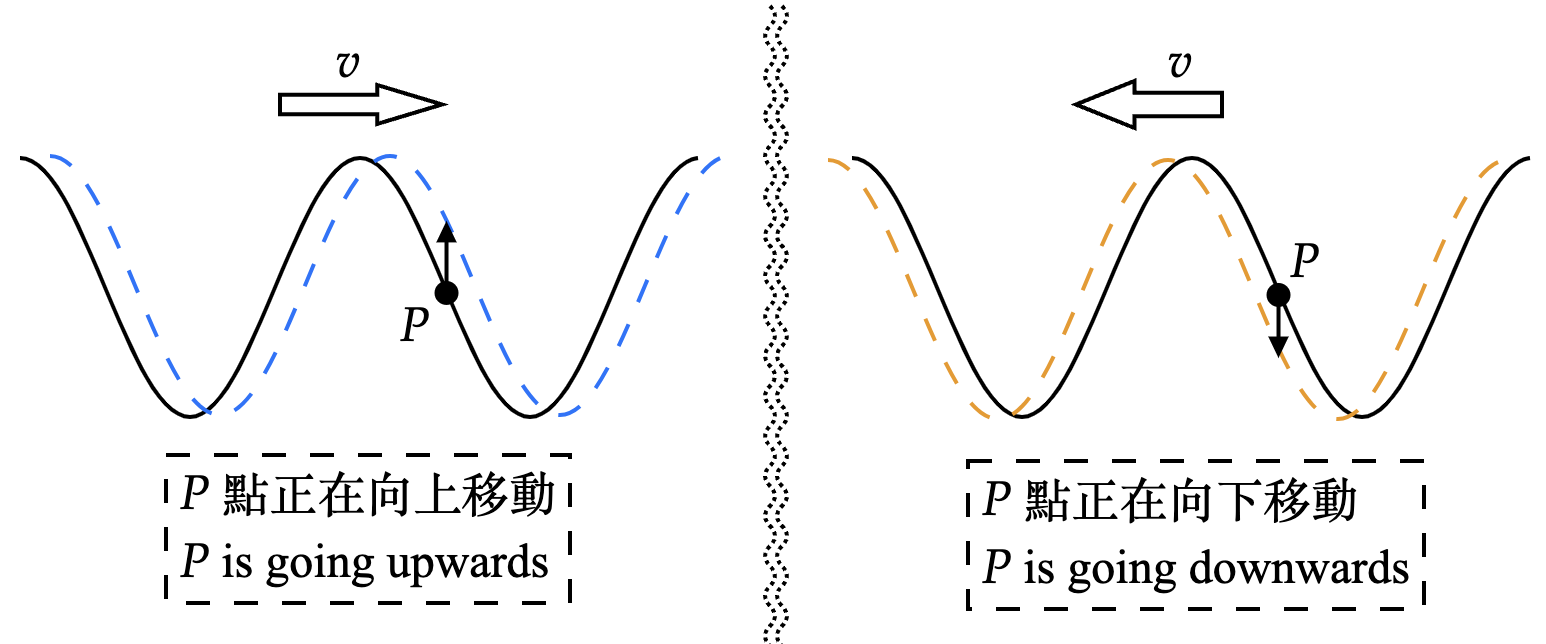
\includegraphics[width=\textwidth]{./img/ch1_2024-05-09-14-58-40.png}\par}
    \begin{itemize}
        \item 注意在同一樣波形,各質點的移動方向取決於行波的傳播方向。
    \end{itemize}
\end{frame}

% \begin{frame}
%     \frametitle{行波Travelling waves}
%     \par{\par\centering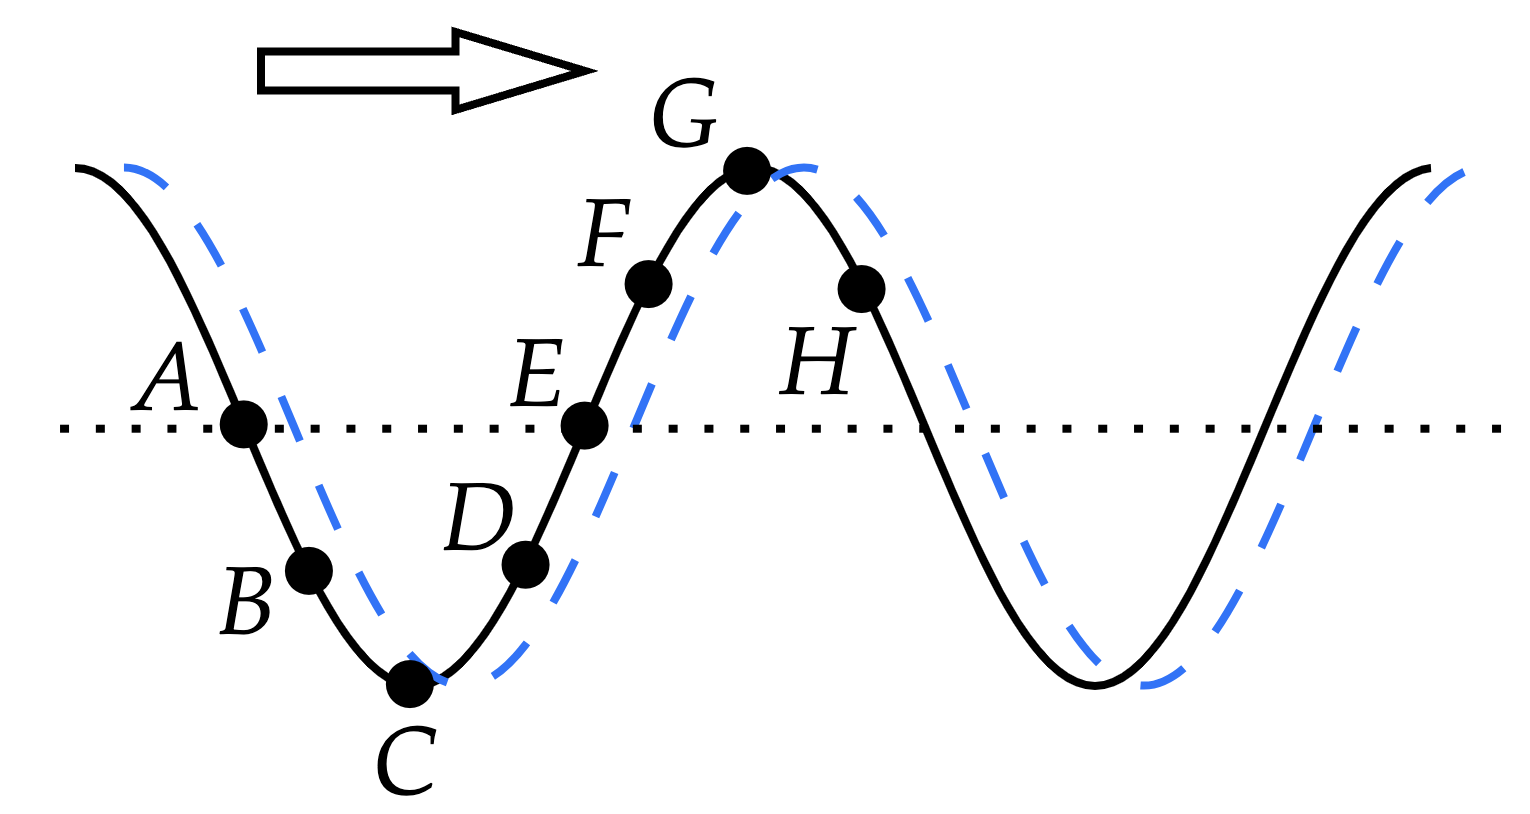
\includegraphics[width=.5\textwidth]{./img/ch1_2024-05-09-15-04-33.png}\par}
%     \begin{table}[]
%         \begin{tabular}{l|l|l|l|l}
%             \makecell{速率最大 \\greatest speed} & \makecell{速度最大\\greatest velocity} & \makecell{加速度最大\\greatest acceleration}   & \makecell{動能最大\\greatest KE} & \makecell{勢能最大\\greatest PE} \\
%             \hline
%              &  &  &  &    \\
%              &  &  &  &    \\
%             \hline
%             \makecell{速率最小 \\lowest speed} & \makecell{速度最小\\lowest velocity} & \makecell{加速度$=0$\\acceleration $=0$} & \makecell{動能最小\\lowest KE} & \makecell{勢能最小\\lowest PE} \\
%             \hline
%              &  &  &  &    \\
%              &  &  &  &    \\
%             % \hline
%         \end{tabular}
%     \end{table}
% \end{frame}


\begin{frame}
    \frametitle{行波Travelling waves}
    \par{\par\centering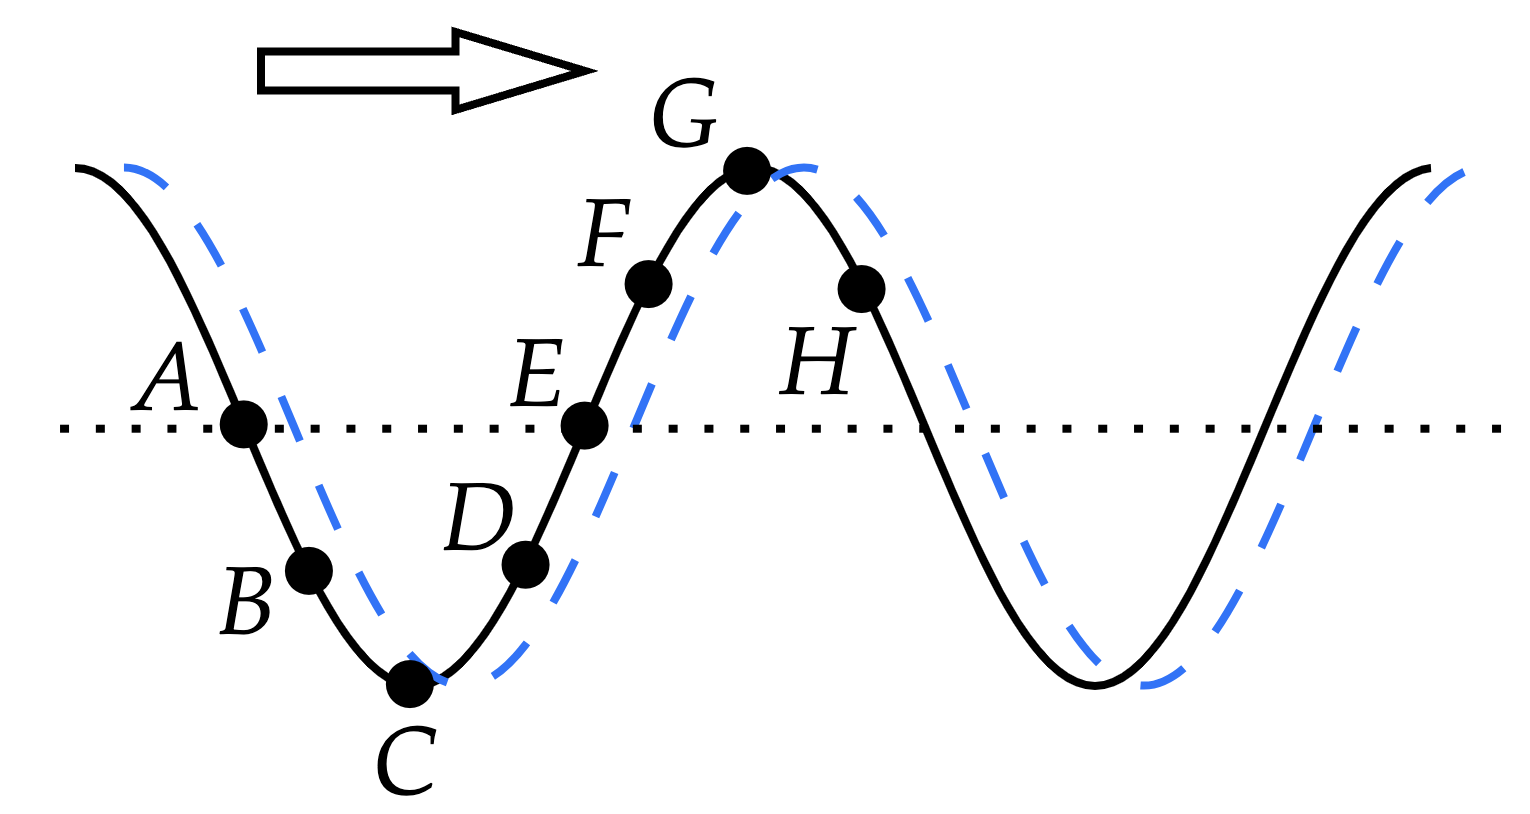
\includegraphics[width=.5\textwidth]{./img/ch1_2024-05-09-15-04-33.png}\par}
    \begin{table}[]
        \begin{tabular}{l|l|l|l}
            \makecell{速度最大量值 \\greatest velocity} & \makecell{加速度最大量值\\greatest magnitude\\of acceleration}   & \makecell{動能最大\\greatest KE} & \makecell{勢能最大\\greatest PE} \\
            \hline
             &  &  &         \\
             &  &  &         \\
            \hline
            \makecell{速度最小量值 \\lowest velocity} & \makecell{加速度$=0$\\acceleration $=0$} & \makecell{動能最小\\lowest KE} & \makecell{勢能最小\\lowest PE} \\
            \hline
             &  &  &         \\
             &  &  &         \\
            % \hline
        \end{tabular}
    \end{table}
\end{frame}

\begin{frame}
    \frametitle{行波Travelling wave}
    \begin{itemize}
        \item 在行波中,每個質點具有相同的能量(KE + PE),和相同的振幅。
        \item 在行波中,波形和能量向前傳播。
        \item 質點只會以平衡位置為中心進行振動。
        \item 質點的移動速率 $\neq$ 行波的速率。
    \end{itemize}


\end{frame}


\begin{frame}
    \frametitle{例題Example}
    \par{\par\centering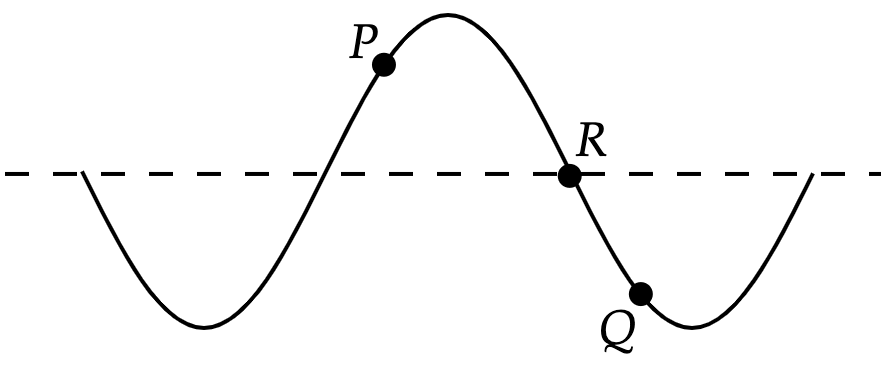
\includegraphics[width=.5\textwidth]{./img/ch1_2024-05-09-15-30-47.png}\par}
    如上圖所示,一道橫行波沿着一根繩子傳播。在圖示時刻,質點$P$正向上移動。下列各項敘述,那一項\textbf{不正確}?
\end{frame}

\begin{frame}[t]{例題Example}
    \begin{tasks}
        \task 這道波正向左移動。
        \task 質點$P$和$Q$以相同振幅振動。
        \task 質點$Q$在圖示時刻正向下移動。
        \task 質點 $R$ 在圖示時刻靜止不動。
    \end{tasks}
\end{frame}






































































































\end{document}